\documentclass[11pt,a4paper]{article}
\usepackage[utf8]{inputenc}
\usepackage[T1]{fontenc}
\usepackage[spanish,es-tabla]{babel}
\usepackage[margin=2.05cm,headheight=16pt,headsep=0.45cm,footskip=0.9cm]{geometry}
\usepackage{lmodern}
\usepackage{microtype}
\usepackage{graphicx}
\usepackage{xcolor}
\usepackage{amsmath,amssymb}
\usepackage{booktabs,tabularx,longtable,array,multirow}
\usepackage[most]{tcolorbox}
\usepackage{float}
\usepackage{enumitem}
\usepackage{titlesec}
\usepackage{fancyhdr}
\usepackage{hyperref}
\usepackage{xurl}
\usepackage{pdfpages}
\usepackage{caption}
\usepackage{setspace}
\definecolor{DarkBlue}{RGB}{20,50,90}
\definecolor{AccentBlue}{RGB}{0,102,180}
\definecolor{BgGrey}{RGB}{245,247,250}
\definecolor{MidGrey}{RGB}{89,101,121}
\definecolor{Gold}{RGB}{179,138,46}
\definecolor{Warn}{RGB}{159,72,40}
\hypersetup{colorlinks=true,linkcolor=AccentBlue,urlcolor=AccentBlue,citecolor=DarkBlue,pdftitle={Expediente completo MCH Río Blanco 100 kW},pdfauthor={Renzo Gabriel Mamani Galindo}}
\setlength{\parindent}{0pt}
\setlength{\parskip}{5pt}
\setstretch{1.04}
\setlist[itemize]{leftmargin=1.2em,itemsep=2pt,topsep=3pt}
\setlist[enumerate]{leftmargin=1.5em,itemsep=2pt,topsep=3pt}
\pagestyle{fancy}
\fancyhf{}
\fancyhead[L]{\small\color{MidGrey}MCH Río Blanco · Expediente de prefactibilidad}
\fancyhead[R]{\small\color{MidGrey}Renzo G. Mamani Galindo}
\fancyfoot[L]{\small\color{MidGrey}Centrales Hidroeléctricas · Grupo A}
\fancyfoot[R]{\small\color{MidGrey}Página \thepage}
\renewcommand{\headrulewidth}{0.4pt}
\renewcommand{\headrule}{\hbox to\headwidth{\color{AccentBlue}\leaders\hrule height \headrulewidth\hfill}}
\renewcommand{\footrulewidth}{0pt}
\titleformat{\section}{\Large\bfseries\color{DarkBlue}}{}{0pt}{}
\titleformat{\subsection}{\large\bfseries\color{AccentBlue}}{}{0pt}{}
\titleformat{\subsubsection}{\normalsize\bfseries\color{DarkBlue}}{}{0pt}{}
\titlespacing*{\section}{0pt}{12pt}{6pt}
\titlespacing*{\subsection}{0pt}{9pt}{3pt}
\titlespacing*{\subsubsection}{0pt}{7pt}{2pt}
\captionsetup{font=small,labelfont=bf}
\newtcolorbox{resumenbox}[1][]{colback=BgGrey,colframe=AccentBlue,boxrule=.6pt,arc=2mm,left=2mm,right=2mm,top=1mm,bottom=1mm,#1}
\newtcolorbox{alertabox}[1][]{colback=BgGrey,colframe=Warn,boxrule=.7pt,arc=2mm,left=2mm,right=2mm,top=1mm,bottom=1mm,#1}
\newtcolorbox{azulbox}[1][]{colback=DarkBlue,colframe=DarkBlue,coltext=white,boxrule=.4pt,arc=2mm,left=2mm,right=2mm,top=2mm,bottom=2mm,#1}
\newcommand{\capitulo}[2]{\clearpage\section*{CAPÍTULO #1. #2}\addcontentsline{toc}{section}{Capítulo #1. #2}}
\newcommand{\apendice}[2]{\clearpage\section*{ANEXO #1. #2}\addcontentsline{toc}{section}{Anexo #1. #2}}
\newcolumntype{Y}{>{\raggedright\arraybackslash}X}
\renewcommand{\arraystretch}{1.15}
\begin{document}
\thispagestyle{empty}

% PORTADA, en el estilo visual de referencia
\begin{tcolorbox}[colback=DarkBlue,colframe=DarkBlue,arc=3mm,boxrule=0pt,top=7mm,bottom=7mm,left=5mm,right=5mm]
\color{white}\centering
{\Large\bfseries UNIVERSIDAD NACIONAL DEL ALTIPLANO}\par\vspace{2mm}
{\large ASIGNATURA: CENTRALES HIDROELÉCTRICAS}\par\vspace{8mm}
{\Huge\bfseries EXPEDIENTE TÉCNICO}\par\vspace{2mm}
{\LARGE MICROCENTRAL HIDROELÉCTRICA}\par
{\LARGE\bfseries RÍO BLANCO — 100 kW}\par\vspace{4mm}
{\large Estudio de prefactibilidad · Capítulos I–XI y anexos}\par
\end{tcolorbox}
\vspace{3mm}
\begin{tabularx}{\textwidth}{>{\bfseries}p{4.8cm}Y}
Estudiante: & Renzo Gabriel Mamani Galindo\\
Asignatura: & Centrales Hidroeléctricas\\
Docente responsable: & Meza Marocho Gregorio\\
Sección: & Grupo A\\
Universidad: & Universidad Nacional del Altiplano\\
Ubicación del proyecto: & Ollachea, Carabaya, Puno\\
Fecha: & 16 de octubre de 2026\\
\end{tabularx}
\vspace{3mm}\hrule\vspace{4mm}
\begin{resumenbox}[title=Estado y alcance]
Este expediente integra los estudios y anexos disponibles en la carpeta del proyecto con la secuencia de capítulos solicitada. Es un documento académico de \textbf{prefactibilidad}. Las series, coordenadas, metrados, costos, equipos, planos y permisos contienen supuestos y referencias de gabinete; no son una aprobación de disponibilidad hídrica ni ingeniería apta para construcción. Los anexos de origen se reproducen como respaldo documental y no se consideran validados por su sola inclusión.
\end{resumenbox}
\vfill
\begin{center}\small\color{MidGrey}Documento de trabajo para revisión académica y técnica\end{center}
\clearpage

\section*{RESUMEN EJECUTIVO}
La alternativa considera una microcentral hidroeléctrica de pasada con salto bruto de 115 m y caudal de diseño supuesto de 0,125 m$^3$/s. El esquema comprende captación, desarenador, canal de aducción de 450 m, cámara de carga, tubería forzada de 380 m y 250 mm de diámetro adoptado, turbina Pelton de dos inyectores, generador síncrono de referencia de 125 kVA y evacuación eléctrica conceptual a 10 kV.

El análisis de la serie de trabajo 2014--2023 calcula Qmedio = 0,523 m$^3$/s y Q95 = 0,126 m$^3$/s. Al restar la reserva supuesta de 0,030 m$^3$/s quedan 0,096 m$^3$/s en Q95, por debajo de Qd. La serie no tiene trazabilidad primaria acreditada en este paquete; la energía modelada de 862,92 MWh/año no constituye energía firme.

La cadena de potencia reporta 130,20 kW hidráulicos, 114,58 kW mecánicos, 106,56 kW a bornes y 104,43 kW después del transformador. Un generador de 125 kVA a cos $\varphi=0,80$ corresponde a 100 kW activos; falta coordinar potencia y límite de operación. La estimación CAPEX es USD 245 800 sin cotizaciones verificables. Los indicadores económicos son ilustrativos.

\begin{resumenbox}[title=Hallazgos que gobiernan la siguiente decisión]
\begin{itemize}
\item Validar registros de caudal, balance mensual, derechos de agua y caudal ecológico.
\item Reconciliar eficiencia global, pérdidas localizadas y diámetro económico de la conducción.
\item Armonizar turbina, generador, transformador, protecciones y punto de conexión.
\item Levantar topografía y geotecnia; revisar crecidas, sedimentos, servidumbres e impactos.
\item Actualizar metrados y presupuesto con planos y cotizaciones antes de decidir factibilidad.
\end{itemize}
\end{resumenbox}

\section*{CONTROL DOCUMENTAL Y REGISTRO DE REVISIONES}
\begin{table}[H]\centering\small
\begin{tabularx}{\textwidth}{p{1.2cm}p{2.1cm}p{3.0cm}Y}
\toprule Rev. & Fecha & Descripción & Estado / responsable\\\midrule
0 & 2024--2026 & Documentos base de prefactibilidad, scripts, anexos y figuras disponibles en el repositorio. & Material fuente; fechas/autores de varias piezas no acreditan campañas de campo.\\
1 & 16/10/2026 & Integración en los capítulos I--XI, incorporación de tablas de estudios y revisión de consistencia documental. & Preparó Renzo Gabriel Mamani Galindo para la asignatura; revisión de ingeniería y aprobación institucional pendientes.\\
\bottomrule
\end{tabularx}\caption{Historial de elaboración de esta compilación. No equivale a aprobación o firma de ingeniería.}\end{table}

\section*{MATRIZ DE OBSERVACIONES Y REVISIONES TÉCNICAS}
\begin{longtable}{p{.65cm}p{3.4cm}p{4.0cm}p{5.0cm}}
\toprule ID & Observación & Efecto en el expediente & Acción de cierre\\\midrule
\endhead
R1 & Procedencia de serie hidrológica & No permite acreditar disponibilidad ni energía firme. & Obtener archivos primarios, estación, curvas de gasto, aforos, control de calidad y metadatos; recalcular CDC.\\
R2 & Q95 menos Qeco & 0,126--0,030 = 0,096 m$^3$/s, inferior a Qd=0,125 m$^3$/s. & Revisar caudal ambiental con ANA y optimizar potencia/diseño con balance mensual.\\
R3 & Potencia nominal & 104,43 kW calculados frente a 100 kW activos de 125 kVA a cos $\varphi=0,8$. & Seleccionar conjunto coordinado, factor de potencia, límites y control de exportación.\\
R4 & Pérdidas singulares & Anexo C asocia $\Sigma K=1,85$ con $h_m=1,15$ m; aritméticamente da cerca de 0,61 m. & Recalcular accesorios y salto neto con el trazado definitivo.\\
R5 & Diámetro económico & Documentos reportan 0,246 m y 0,413 m frente a 0,250 m adoptado. & Rehacer comparación costo de tubería/energía/presión con bases explícitas.\\
R6 & Eficiencia global & El modelo anual usa 0,73; otro módulo informa 0,7405; el producto punto a punto es aproximadamente 0,802. & Unificar pérdidas y eficiencias antes de recalcular energía e indicadores.\\
R7 & Campo y geotecnia & No se acredita levantamiento, campaña geotécnica, crecidas ni replanteo. & Ejecutar los TDR de Gate 0 y desarrollar estudios de factibilidad.\\
R8 & Costos y demanda & CAPEX, tarifas, usuarios y usos productivos no cuentan con evidencia contractual. & Obtener cotizaciones, encuesta de carga, costos operativos y acuerdo de compra/conexión.\\
\bottomrule
\end{longtable}

\tableofcontents
\clearpage

% CAPÍTULO I
\capitulo{I}{MEMORIA DESCRIPTIVA}
\subsection*{1.1 Denominación y datos generales}
El proyecto académico se denomina \textbf{Microcentral Hidroeléctrica Río Blanco, 100 kW}. El ámbito de estudio se indica en el distrito de Ollachea, provincia de Carabaya, departamento de Puno, en el sistema hidrográfico asociado al río Inambari. El eje de captación, restitución, cotas, coordenadas, límites de predios y accesos son referencias del paquete y deben verificarse antes de ser usados para replanteo o trámite.

\subsection*{1.2 Antecedentes, problema y justificación}
La generación hidroeléctrica de pequeña escala puede complementar el servicio local y habilitar usos productivos si existe recurso hídrico compatible, demanda y conexión viable. La carpeta describe como posibilidades el procesamiento de café y cacao, la cadena de frío para acuicultura, transformación de fibra, bombeo y servicios rurales. En ausencia de encuestas de demanda, acuerdos comunitarios y condiciones de venta, estos beneficios se consideran hipótesis que requieren consulta local.

\subsection*{1.3 Objetivos}
\textbf{Objetivo general:} evaluar a nivel de prefactibilidad una alternativa conceptual de microcentral de pasada de 100 kW en Río Blanco. \textbf{Objetivos específicos:} describir captación, conducción y generación; revisar la disponibilidad hídrica y los cálculos hidráulicos; evaluar la compatibilidad preliminar de Pelton, generador y evacuación; ordenar los documentos técnicos; identificar los datos, permisos y estudios necesarios para decidir si se avanza a factibilidad.

\subsection*{1.4 Localización, cartografía y contexto físico}
La localización política reportada es Ollachea--Carabaya--Puno. El material base presenta una cuenca de 28,45 km$^2$, perímetro de 24,12 km, elevación media 3 180 m s.n.m. y divisoria máxima de 4 150 m s.n.m.; son parámetros extraídos de cartografía de trabajo, no un levantamiento hidrológico/geodésico certificado. El salto bruto de 115 m corresponde a cotas conceptuales de 2 420,0 y 2 302,8 m s.n.m. La comprobación requiere nivelación y control horizontal/vertical en campo.

\subsection*{1.5 Descripción del aprovechamiento}
La alternativa es de pasada. Una captación de fondo derivaría el caudal autorizado; un desarenador reduciría la carga de sólidos; el canal de aducción conduciría el agua a una cámara de carga; la tubería forzada entregaría presión a la turbina Pelton y el agua retornaría al río. No se plantea un embalse de regulación estacional. El caudal ecológico de 30 L/s es un dato de cálculo, no un valor aprobado.

\begin{table}[H]\centering\small
\begin{tabularx}{\textwidth}{p{2.5cm}p{5.0cm}Y}
\toprule Componente & Parámetros de referencia & Condición de prefactibilidad\\\midrule
Captación & Tipo tirolesa; rejilla Coanda; azud con cresta reportada 4 m; capacidad reportada 144 L/s. & Capacidad de avenida, socavación, sedimentos y fundación sin verificación.\\
Desarenador & Dos naves de 8,0 m × 0,70 m × 1,10 m; partícula objetivo 0,20 mm. & Recalcular con granulometría y caudal; confirmar purga y descarga.\\
Canal & 450 m; sección rectangular de base 0,50 m; altura total 0,60 m. & Eje, pendiente, estabilidad y filtración pendientes.\\
Cámara de carga & Volumen útil 22,5 m$^3$; aliviadero y rejilla fina. & Geometría, sumergencia, oleaje y aliviadero por revisar.\\
Tubería & 380 m; 250 mm de diámetro interior adoptado. & Diámetro, presión, espesor, soportes y anclajes pendientes.\\
Casa de máquinas & Pelton horizontal, generador y tablero. & Cimentación, acceso, inundación y geotecnia pendientes.\\
\bottomrule
\end{tabularx}\caption{Descripción funcional de la alternativa; no son dimensiones para construcción.}\end{table}

\subsection*{1.6 Equipo electromecánico y sistema de evacuación}
La alternativa de cálculo considera turbina Pelton horizontal con dos inyectores, caudal total de 125 L/s, salto neto calculado de 106,18 m y velocidad de referencia de 1 200 rpm. El generador de 125 kVA a 400/230 V y 60 Hz es referencial. Se estudia un transformador de 125 kVA y 0,4/10 kV, además de una línea de media tensión reportada de 3,2 km. El punto de conexión, tensión, ruta, protecciones, medición, servidumbres y reglas de operación no están aprobados por la distribuidora.

\subsection*{1.7 Operación, mantenimiento y seguridad}
Durante operación, captación y derivación deben respetar el derecho de uso y el caudal ambiental que se determinen. Las rutinas previstas incluyen limpieza de rejilla, purga del desarenador, revisión del canal y tubería, control de vibración/temperatura y pruebas de protecciones. Los intervalos concretos, personal, repuestos y disponibilidad se definirán con fabricante, estudios de sedimentos y plan de operación. El sistema debe contar con parada de emergencia, resguardos y procedimientos de seguridad.

\subsection*{1.8 Gestión ambiental, social y permisos}
No se cuenta con clasificación ambiental aprobada ni instrumento de gestión ambiental. Deben evaluarse el tramo intervenido, sedimentos, hábitat acuático, calidad de agua, caudal ecológico, accesos, servidumbres, residuos, ruido, vegetación y aceptación local. La categoría y el instrumento aplicable deben ser definidos por la autoridad competente según el alcance real y la normativa vigente. No se presume que los permisos de agua, obras, ambientales, arqueológicos, prediales ni de conexión estén obtenidos.

\subsection*{1.9 Alcance, exclusiones y limitaciones}
Esta memoria ordena una base académica de prefactibilidad. No es expediente definitivo, diseño de detalle, especificación de compra, presupuesto contractual, permiso ni garantía de potencia/energía. La serie hidrológica carece de trazabilidad primaria acreditada. Coordenadas, topografía, geotecnia, avenida, sedimentos, demanda, conexión y costos son datos de trabajo que deben reemplazarse o validarse.

% CAPÍTULO II
\capitulo{II}{CÁLCULOS JUSTIFICATIVOS}
\subsection*{2.1 Bases de cálculo}
Las ecuaciones se reproducen para revisar consistencia y orden de magnitud. La reproducibilidad matemática no acredita calidad de las entradas. Se adoptan $g=9,81$ m/s$^2$, $\rho=1\,000$ kg/m$^3$, $Q_d=0,125$ m$^3$/s, $Q_{eco}=0,030$ m$^3$/s, $H_b=115$ m, $L=380$ m, $D=0,250$ m y rugosidad absoluta de acero de 0,045 mm. Las eficiencias nominales de cálculo son $\eta_t=0,88$, $\eta_g=0,93$ y $\eta_{tr}=0,98$.

\subsection*{2.2 Régimen hídrico y caudal de diseño}
La curva de duración se calcula por frecuencia empírica de Weibull, $P=m/(N+1)\times100$, donde $m$ es rango descendente y $N=3\,652$. La serie diaria entre 2014 y 2023 arroja los valores siguientes. La procedencia de los datos y la equivalencia de la serie con aforos observados no se acreditan en el paquete.
\begin{table}[H]\centering\small
\begin{tabular}{lrrr}\toprule Persistencia & Caudal de río (m$^3$/s) & Reserva usada (m$^3$/s) & Disponible estimado (m$^3$/s)\\\midrule
Q10 & 1,094 & 0,030 & 1,064\\ Q25 & 0,748 & 0,030 & 0,718\\ Q50 & 0,333 & 0,030 & 0,303\\ Q75 & 0,210 & 0,030 & 0,180\\ Q78 & 0,198 & 0,030 & 0,168\\ Q85 & 0,173 & 0,030 & 0,143\\ Q90 & 0,152 & 0,030 & 0,122\\ Q95 & 0,126 & 0,030 & 0,096\\\bottomrule
\end{tabular}\caption{Resultados del modelo de serie provisional; no constituyen disponibilidad acreditada.}\end{table}
En Q95 el disponible estimado queda 23,2\% por debajo de Qd. La serie debe auditarse, completar con datos primarios, revisar curva de gasto y balance mensual, y determinar el caudal ecológico por metodología aplicable. El Qeco de 30 L/s es hipótesis; no es determinación ANA.

\subsection*{2.3 Crecidas de referencia}
El informe base ajusta máximos anuales a Gumbel tipo I. Los valores reportados son $Q_{10}=3,04$, $Q_{25}=3,34$, $Q_{50}=3,56$, $Q_{100}=3,77$ y $Q_{500}=4,28$ m$^3$/s. No se dispone aquí de la serie primaria de máximos, pruebas de ajuste, homogeneidad ni análisis de incertidumbre. Estos caudales no se aceptan como diseño de azud/aliviadero hasta reproducir el análisis con datos verificables y criterios de seguridad apropiados.

\subsection*{2.4 Canal a superficie libre: Manning}
Para un canal rectangular, $Q=(1/n)AR_h^{2/3}S_0^{1/2}$. Con $b=0,50$ m, $y=0,331$ m, $n=0,014$ y $S_0=0,0015$, se obtiene $A=by=0,1655$ m$^2$, perímetro mojado $P=b+2y=1,162$ m y radio hidráulico $R_h=A/P=0,1424$ m. El caudal calculado es aproximadamente 0,125 m$^3$/s; la velocidad media $V=Q/A=0,755$ m/s y el Froude $Fr=V/\sqrt{gy}\approx0,419$, subcrítico. Deben comprobarse borde libre, transiciones, juntas, filtraciones y estabilidad de ladera.

\subsection*{2.5 Tubería forzada: velocidad y pérdidas}
Por continuidad, $V=Q/(\pi D^2/4)=2,546$ m/s y $Re\approx5,18\times10^5$. Para $f=0,0153$, Darcy--Weisbach da $h_f=f(L/D)(V^2/2g)=7,67$ m. El Anexo C y el informe base asignan $h_m=1,15$ m a $\Sigma K=1,85$; sin embargo, $\Sigma K(V^2/2g)$ produce cerca de 0,61 m. Se reproduce $h_m=1,15$ m únicamente para conservar el salto neto de referencia: $h_{tot}=8,82$ m y $H_n=115-8,82=106,18$ m. El cálculo deberá rehacerse con accesorios, longitudes, rugosidad, rejilla, válvula y codos definitivos.

El diámetro económico presenta otra inconsistencia: el informe base reporta 0,246 m, mientras que la revisión de cálculo de capítulos I--II indica aproximadamente 0,413 m. Se adopta 0,250 m como alternativa inicial, no como diámetro óptimo. La selección económica compara inversión, energía perdida, presión, fabricación, instalación y anclajes.

\subsection*{2.6 Potencia de turbina y cadena de conversión}
La potencia hidráulica es $P_h=\rho gQH_n/1000=130,20$ kW. Con $\eta_t=0,88$, $P_{eje}=114,58$ kW; con $\eta_g=0,93$, $P_{bornes}=106,56$ kW; con $\eta_{tr}=0,98$, $P_{salida}=104,43$ kW. Se reportan dos inyectores con $Q_j=0,0625$ m$^3$/s cada uno, velocidad de chorro de 44,27 m/s, diámetro de chorro de 42,4 mm, diámetro primitivo de 324,1 mm y 19 cucharas. Son dimensiones de cálculo, no ficha garantizada por fabricante.

\subsection*{2.7 Compatibilidad generador y transformador}
$P_{activa}=S\cos\varphi$. Para $S=125$ kVA y $\cos\varphi=0,80$, la potencia activa nominal es 100 kW. El resultado de 104,43 kW supera esa referencia en 4,43 kW (4,43\%). Se requiere ajustar caudal/punto de operación, limitar potencia o seleccionar un conjunto con curvas y márgenes certificados. Para transformador trifásico de 125 kVA, $I=S/(\sqrt3V)$ da aproximadamente 180,4 A a 0,4 kV y 7,22 A a 10 kV. No incluye cortocircuito ni coordinación de protecciones.

\subsection*{2.8 Transitorio hidráulico y espesor indicativo}
Con celeridad reportada $a=1\,195,79$ m/s, el tiempo crítico es $t_c=2L/a=0,636$ s. Para cierre supuesto de 4 s y velocidad inicial 2,546 m/s, la aproximación de cierre lento da $\Delta H=2LV/(gt)=49,32$ m.c.a.; $H_{max}=H_b+\Delta H=164,32$ m.c.a., aproximadamente 16,11 bar. El espesor reportado de 3,11 mm incorpora una reserva de corrosión de 1,5 mm y esfuerzo admisible supuesto de 125 MPa. No reemplaza código de diseño ni verificaciones de vacío, soldadura, tolerancias, fatiga, soportes, presión de prueba, maniobras de emergencia y anclajes.

\subsection*{2.9 Energía y economía reproducible}
El modelo anual informa 862,92 MWh y factor de planta 98,51\%, con eficiencia global simplificada 0,73. Otro módulo informa 0,7405 y la cadena de eficiencias punto a punto da aproximadamente 0,802. El modelo usa CAPEX USD 245 800, OPEX 3\% anual del CAPEX, tarifa USD 0,075/kWh, 25 años y descuento 10\%. La corrida de referencia reporta VAN USD 274 741,65, TIR 23,20\%, retorno simple 4,29 años, LCOE USD 39,90/MWh y B/C 1,88. Estos son resultados condicionados a entradas no validadas y no acreditan energía firme, tarifa contratada ni bancabilidad.

% CAPÍTULO III
\capitulo{III}{ESPECIFICACIONES TÉCNICAS DE SUMINISTRO DE MATERIALES}
\subsection*{3.1 Reglas generales de compra}
La compra se realizará contra fichas aprobadas, planos coordinados, características garantizadas, inspección y aceptación documentada. Todo material deberá llevar identificación de fabricante, lote, certificados, manuales, planos, repuestos recomendados, instrucciones de transporte/almacenamiento y garantía. Desviaciones requieren evaluación escrita. La lista siguiente es base de requerimientos, no especificación contractual.
\begin{table}[H]\centering\small
\begin{tabularx}{\textwidth}{p{2.4cm}p{5.1cm}Y}\toprule Suministro & Datos de referencia & Información/ensayos a exigir\\\midrule
Concreto y agregados & Ciclópeo $f'c=175$ kg/cm$^2$; armado $f'c=210$ kg/cm$^2$ según APU. & Diseño de mezcla, fuente y granulometría de agregados, probetas, curado y registro de vaciado.\\
Acero de refuerzo & APU indica $f_y=4\,200$ kg/cm$^2$, grado 60. & Certificados, colada, diámetro, peso, doblado y trazabilidad.\\
Tubería & Referencia ASTM A36; diámetro interior 250 mm; 380 m; espesores preliminares 4,75/6,35 mm en APU. & Clase de presión final, tolerancia, material, soldadura, END, revestimiento, prueba y documentación.\\
Rejillas/compuertas & Rejilla Coanda; espaciamiento reportado 25 mm y rejilla fina en cámara. & Geometría, cargas, corrosión, pérdida de carga, maniobra, limpieza y material certificado.\\
Turbina Pelton & Dos inyectores; CA6NM de referencia; 1 200 rpm. & Curvas garantizadas, eficiencia, embalamiento, vibración, materiales, boquillas y protocolos FAT.\\
Generador/AVR & 125 kVA; 400/230 V; 60 Hz; brushless referencial. & kW nominales a FP declarado, límites térmicos, aislamiento, excitación, AVR y pruebas.\\
ELC/tablero & ELC 120 kW de referencia, tablero digital y protecciones. & Coordinación de carga, disipación térmica, lógica de control, cortocircuito y pruebas funcionales.\\
Transformador/línea & 125 kVA, 0,4/10 kV y línea reportada 3,2 km. & Nivel de red acordado, impedancia, pérdidas, aislamiento, grupo vectorial, accesorios y aceptación del operador.\\
\bottomrule\end{tabularx}\caption{Matriz de suministro preliminar.}\end{table}

\subsection*{3.2 Recepción y aseguramiento de calidad}
El plan de inspección separará revisión documental, inspección visual/dimensional, pruebas de fábrica y pruebas de recepción en sitio. Para materiales civiles se controlarán lotes, certificados y probetas; para tubería, certificados, ovalidad, espesor, soldadura, END y recubrimiento; para equipos, placa, serie, curvas y resultados de rutina; para tableros y transformador, protocolos eléctricos y de protección. La prueba de aceptación debe acordarse antes de emitir orden de compra.

% CAPÍTULO IV
\capitulo{IV}{ESPECIFICACIONES TÉCNICAS DE MONTAJE}
\subsection*{4.1 Condiciones previas}
Antes de movilizar, aprobar planos de detalle, permisos, accesos, servidumbres, zona de acopio, plan de seguridad y salud, plan de manejo ambiental, control topográfico, inspección de materiales y gestión de desvío temporal del río. El trazo y las cotas se comprobarán con levantamiento de campo. Ningún dato de coordenadas del repositorio constituye autorización de ingreso o replanteo.

\subsection*{4.2 Secuencia constructiva preliminar}
\begin{enumerate}
\item Replantear ejes y cotas, verificar interferencias, accesos y estabilidad del terreno. Delimitar áreas y registrar condición ambiental de base.
\item Ejecutar captación con manejo temporal de caudal aprobado; preparar fundación y vaciar azud, rejilla y compuertas según planos. Registrar concreto y tolerancias.
\item Construir desarenador, canal y cámara por tramos; revisar pendientes, juntas, hormigón, aliviadero, transición y estanqueidad.
\item Montar tubería y bloques con apoyos/alineamiento aprobados; emplear procedimientos de soldadura calificados, inspecciones no destructivas y recubrimiento especificado.
\item Instalar válvula, turbina, generador y auxiliares; verificar nivelación, alineamiento, holguras, guardas, lubricación, control y drenaje.
\item Instalar transformador, tableros, cables, puesta a tierra y protecciones; ejecutar pruebas de aislamiento, continuidad, relación, fases, disparos y secuencia de maniobras.
\item Comisionar sin carga y con carga por etapas; ensayar parada de emergencia, rechazo de carga, regulación y alarmas. Sincronizar con red solo con autorización.
\end{enumerate}

\subsection*{4.3 Inspección, seguridad y registros}
Las excavaciones, trabajos en cauce, izaje, trabajo en altura, soldadura y energización tendrán procedimientos, permisos y análisis de riesgos por tarea. Se controlarán crecidas, lluvia, acceso, rescate, bloqueo/etiquetado y comunicación. El expediente de calidad reunirá certificados, ensayos, partes diarios, no conformidades, protocolos, planos conforme a obra, manuales y actas. Los procedimientos y criterios de aceptación deben aprobarse en ingeniería de detalle.

% CAPÍTULO V
\capitulo{V}{CRONOGRAMA}
El siguiente programa organiza hitos indicativos desde la autorización de inicio. No es plazo contractual ni fecha prometida de puesta en servicio. La temporada de lluvia, permisos, acceso y disponibilidad de especialistas pueden modificarlo.
\begin{table}[H]\centering\small
\begin{tabularx}{\textwidth}{p{1.0cm}p{4.1cm}p{2.6cm}Y}\toprule Fase & Actividad & Ventana referencial & Hito/condición\\\midrule
1 & Cotización de Gate 0 y coordinación de acceso & Semanas 1--4 & TDR, polígono, responsables y seguridad acordados.\\
2 & Levantamiento topográfico/geodésico & Semanas 5--10 & Ejes, cotas, secciones y control registrados.\\
3 & Auditoría hidrológica, aforos iniciales y reconocimiento geotécnico & Semanas 5--12 & Trabajo de campo con permisos y trazabilidad.\\
4 & Informe Gate 0 y decisión de continuar & Semanas 13--16 & Matriz de incertidumbres, costos y decisión del titular.\\
5 & Campaña hidrológica ampliada y geotecnia de factibilidad & 12 meses o más & Depende del régimen anual, seguridad y aprobación presupuestal.\\
6 & Instrumento ambiental, derechos, conexión e ingeniería de detalle & Por definir & Según requisitos de ANA, MINEM/autoridad ambiental y distribuidora.\\
7 & Contratación, construcción, montaje y puesta en servicio & Por definir & Requiere diseño firmado, permisos, contratos y protocolos.\\
\bottomrule\end{tabularx}\caption{Secuencia de programación a nivel de prefactibilidad.}\end{table}
La ruta crítica se concentra en validación de disponibilidad hídrica y caudal ecológico, geotecnia, punto de conexión y permisos. La decisión de factibilidad debe tomarse después de integrar esos resultados, no por el calendario preliminar.

% CAPÍTULO VI
\capitulo{VI}{METRADO}
Las cantidades de la tabla provienen del APU de referencia y de dimensiones conceptuales. No son cubicaciones de planos aprobados; sirven para revisar orden de magnitud y deben actualizarse con levantamiento, secciones, clase de terreno y planos de detalle.
\begin{longtable}{p{1.25cm}p{6.9cm}p{1.0cm}p{1.25cm}p{2.2cm}}
\caption{Metrados principales del Anexo D (preliminares).}\\
\toprule Ítem & Descripción & Und. & Cantidad & Estado\\\midrule\endfirsthead
\toprule Ítem & Descripción & Und. & Cantidad & Estado\\\midrule\endhead
01.01 & Limpieza, desbroce y trazo topográfico & m$^2$ & 1 500 & APU\\
01.02 & Excavación para azud & m$^3$ & 185 & APU; geotecnia pendiente\\
01.03 & Concreto ciclópeo de azud & m$^3$ & 65 & APU\\
01.04 & Rejilla Coanda & und & 1 & Conceptual\\
01.05 & Compuertas planas de captación/limpia & und & 2 & Conceptual\\
02.01 & Excavación de desarenador & m$^3$ & 120 & APU\\
02.02 & Concreto armado de desarenador & m$^3$ & 32 & APU\\
02.03 & Acero de refuerzo & kg & 2 400 & APU\\
02.04 & Vertederos Sutro y compuertas de purga & glb & 1 & Conceptual\\
03.01 & Excavación de canal a media ladera & m$^3$ & 380 & APU; terreno pendiente\\
03.02 & Concreto canal 0,50×0,60 m & m$^3$ & 115 & APU; secciones pendientes\\
03.03 & Juntas elastoméricas & m & 150 & APU\\
03.04 & Muros/banquetas de protección & m & 90 & APU\\
04.01 & Excavación de cámara de carga & m$^3$ & 95 & APU\\
04.02 & Concreto cámara & m$^3$ & 28 & APU\\
04.03 & Rejilla fina y compuerta & glb & 1 & Conceptual\\
04.04 & Concreto de cuatro bloques de anclaje & m$^3$ & 59 & Geometría pendiente\\
04.05 & Ventilación anti-vacío DN 100 & und & 1 & Referencia\\
05.01 & Penstock, tramo 0--200 m; espesor 4,75 mm propuesto & m & 200 & Presión pendiente\\
05.02 & Penstock, tramo 200--380 m; espesor 6,35 mm propuesto & m & 180 & Presión pendiente\\
05.03 & Juntas Dresser de alta presión & und & 4 & Revisar selección\\
06.01 & Turbina Pelton dos inyectores & und & 1 & Sin proveedor seleccionado\\
06.02 & Válvula esférica de guarda DN 200 & und & 1 & Revisar diámetro\\
06.03 & ELC y banco resistivo 120 kW & und & 1 & Coordinar potencia\\
06.04 & Generador síncrono 125 kVA & und & 1 & Coordinar kW y FP\\
06.05 & Tablero de control/protecciones & und & 1 & Especificar detalle\\
07.01 & Transformador 125 kVA 0,38/10 kV & und & 1 & Red por confirmar\\
07.02 & Línea aérea 10 kV AAAC 35 mm$^2$ & km & 3,2 & Ruta no aprobada\\
07.03 & Malla de puesta a tierra & glb & 1 & Suelo no medido\\
\bottomrule
\end{longtable}

\subsection*{6.1 Criterios de medición}
Excavaciones se medirán por secciones aprobadas y clasificación del material; concreto por volumen colocado/aceptado; acero por peso según planilla; tubería por diámetro, clase y longitud instalada; equipos por unidad recibida y comisionada; línea por ruta y estructuras. Bases de contratación definirán sobreexcavación, desperdicios, transporte, botaderos, restitución y pagos.

% CAPÍTULO VII
\capitulo{VII}{PLANOS Y LÁMINAS DE DETALLE}
Las figuras disponibles son representaciones de prefactibilidad y no tienen valor de replanteo ni de planos IFC. Los mapas a continuación ayudan a explicar la ubicación general, el esquema de obras y la conducción. Las cotas, ejes, coordenadas, distancias, servidumbres y secciones deben verificarse por levantamiento profesional.
\begin{figure}[H]\centering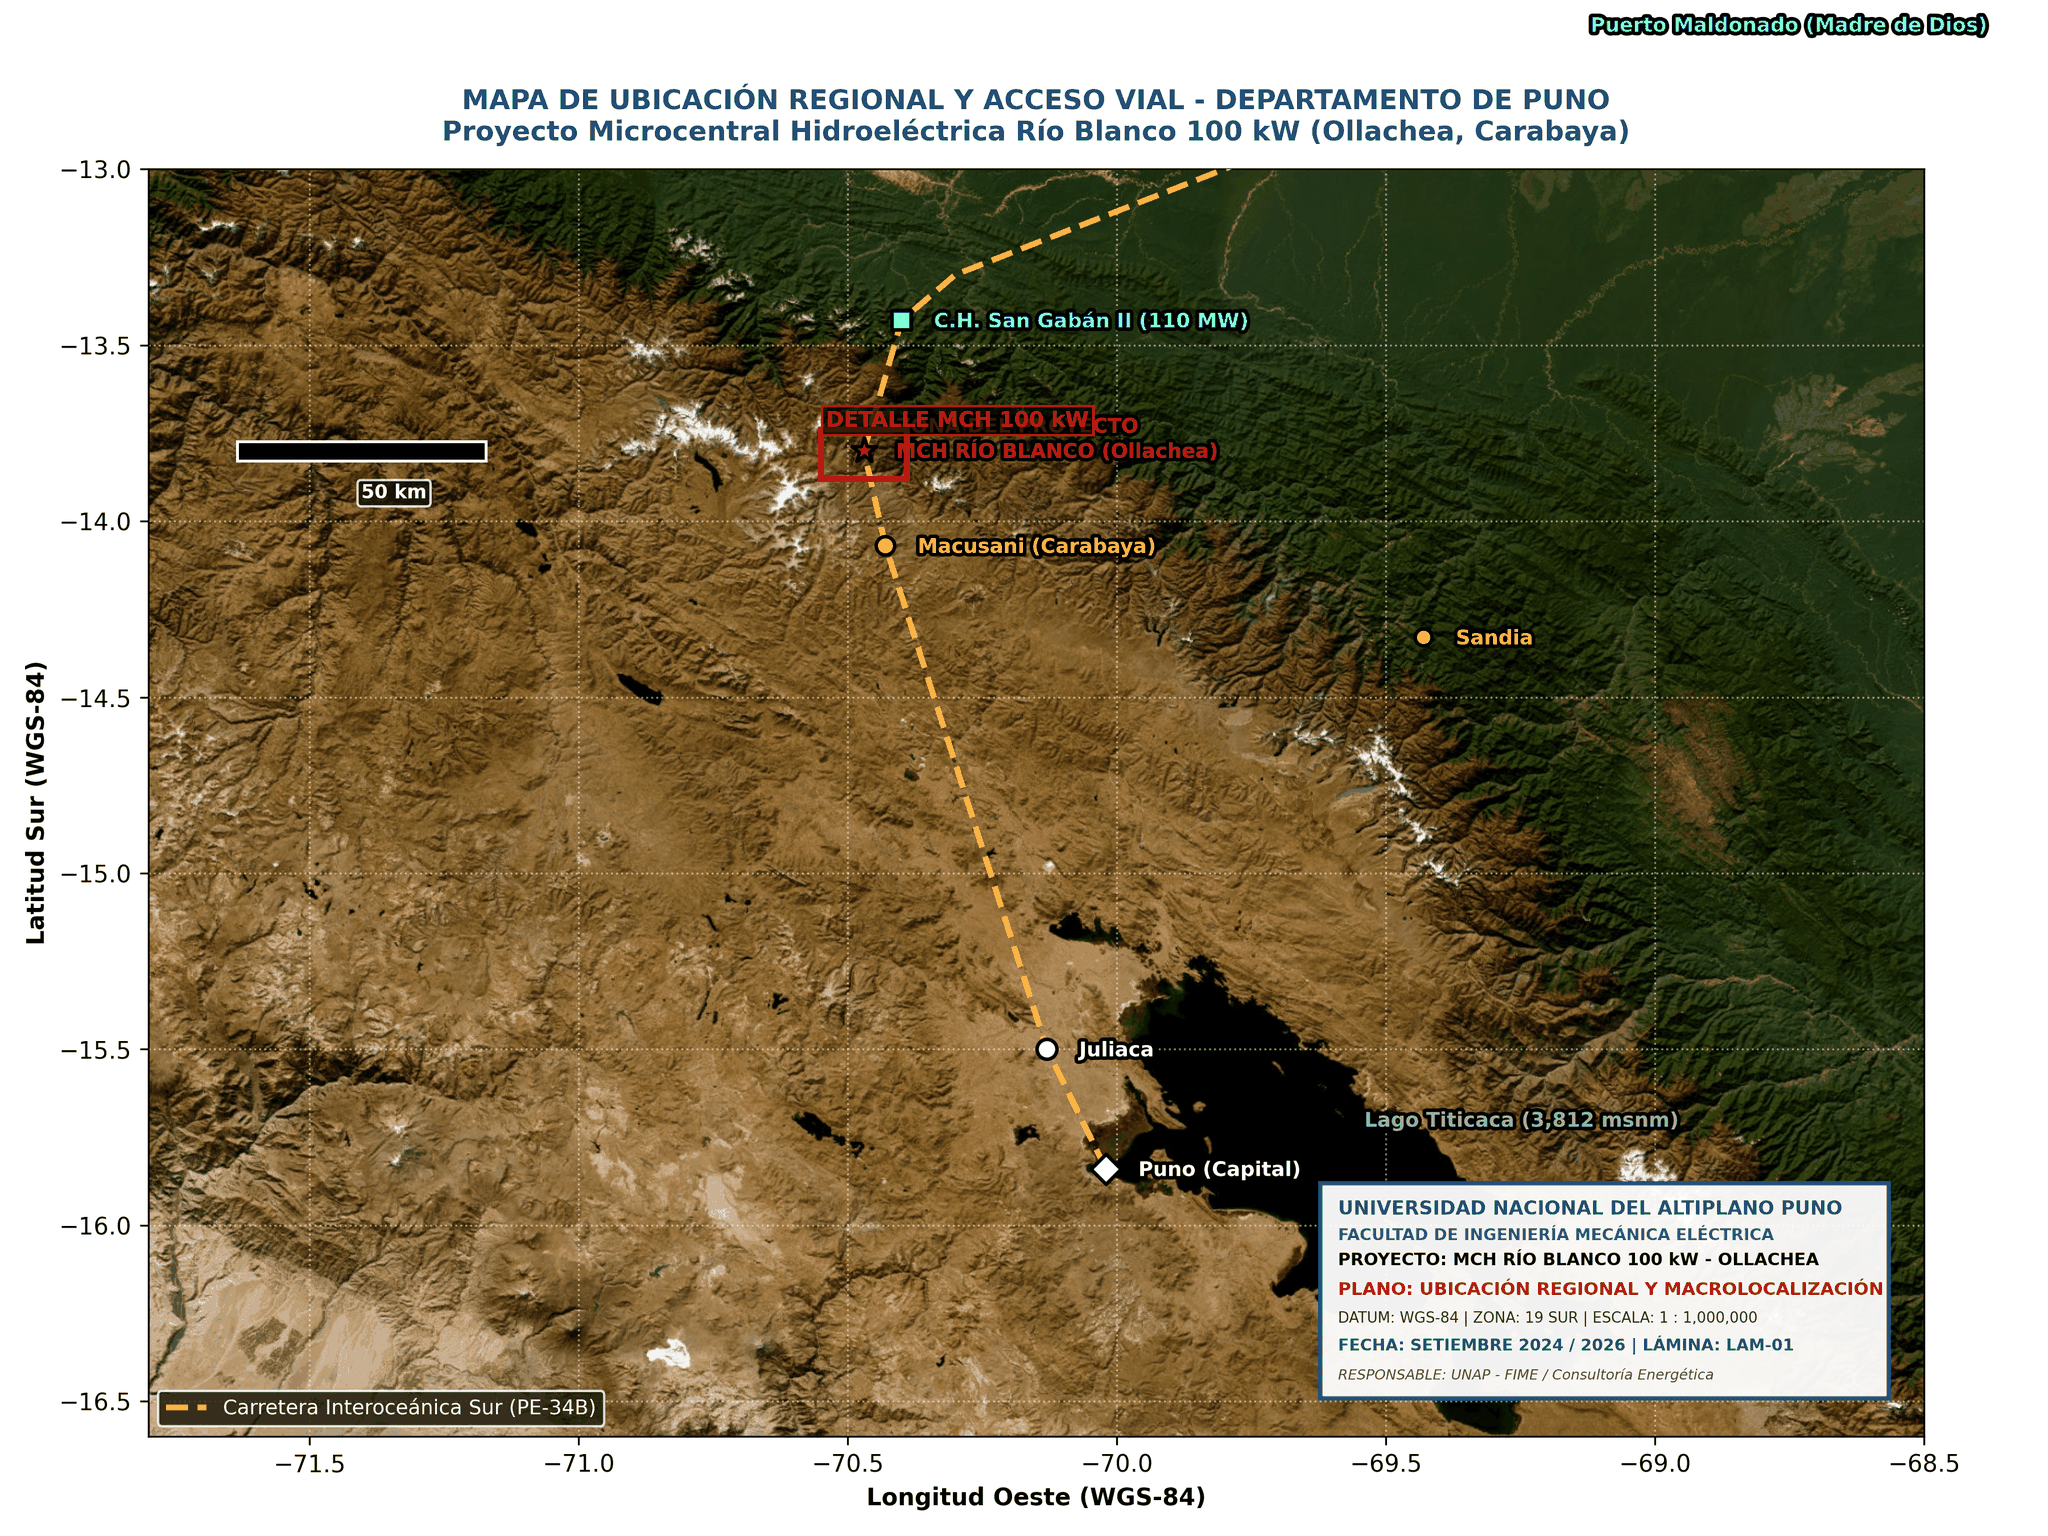
\includegraphics[width=.82\textwidth]{../04 Mapas/Mapa_01_Ubicacion_Regional_Puno.png}\caption{Ubicación regional de referencia; comprobar coordenadas y emplazamiento.}\end{figure}
\begin{figure}[H]\centering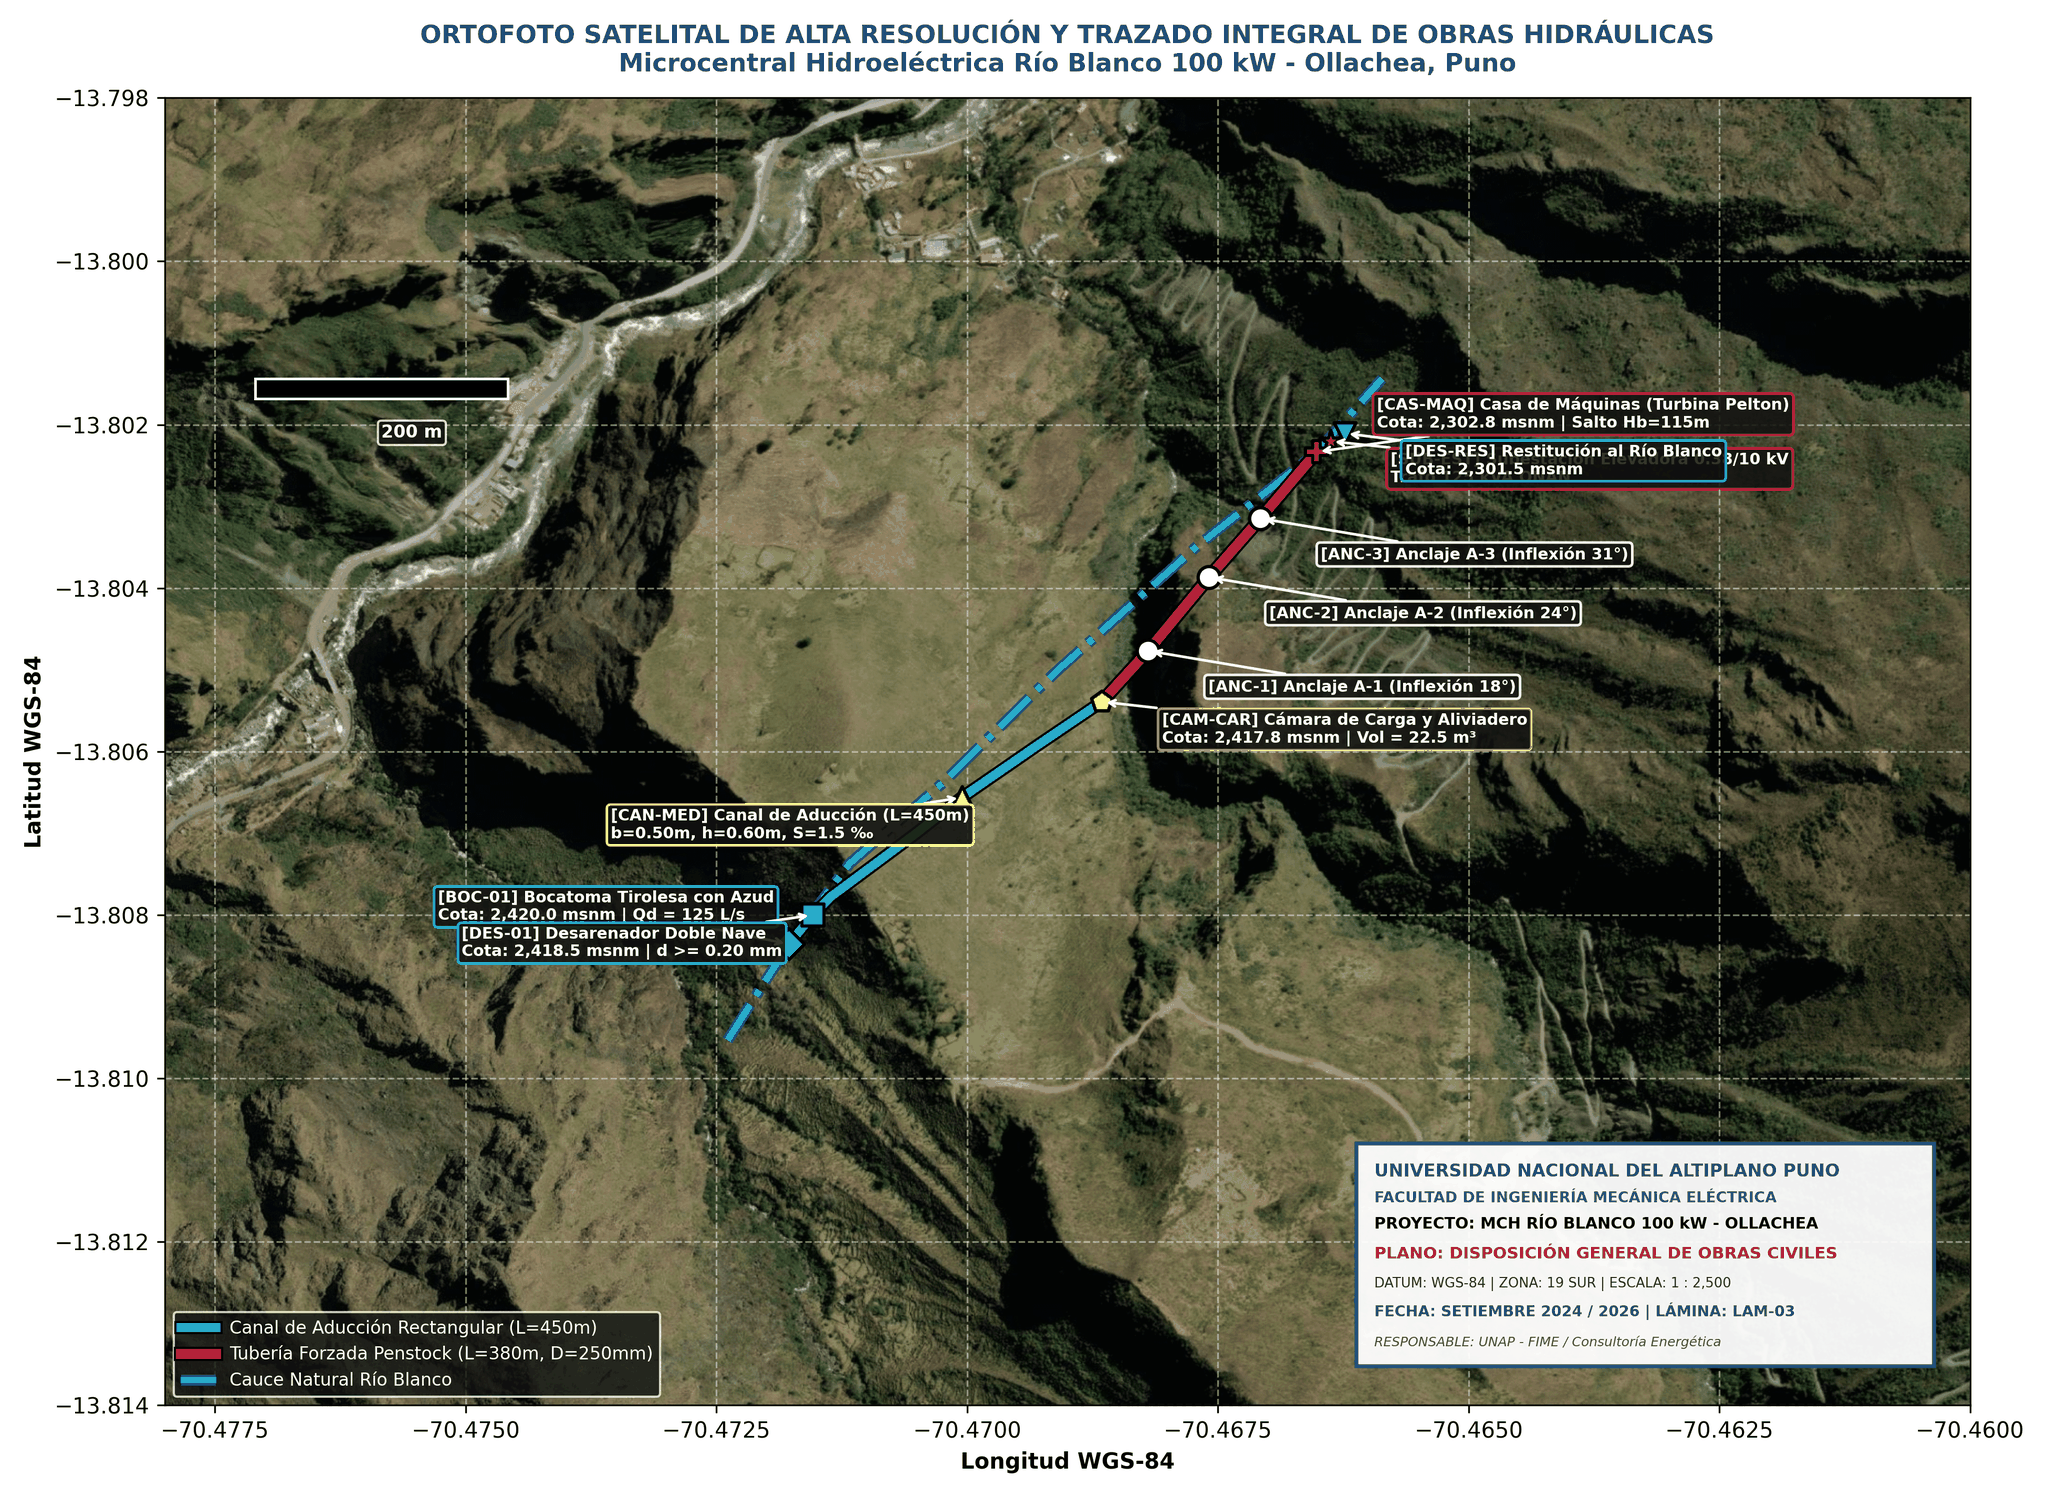
\includegraphics[width=.89\textwidth]{../04 Mapas/Mapa_03_Esquema_Obras_Hidraulicas_Trazo.png}\caption{Esquema conceptual de captación, conducción y restitución; no replanteable.}\end{figure}
\begin{figure}[H]\centering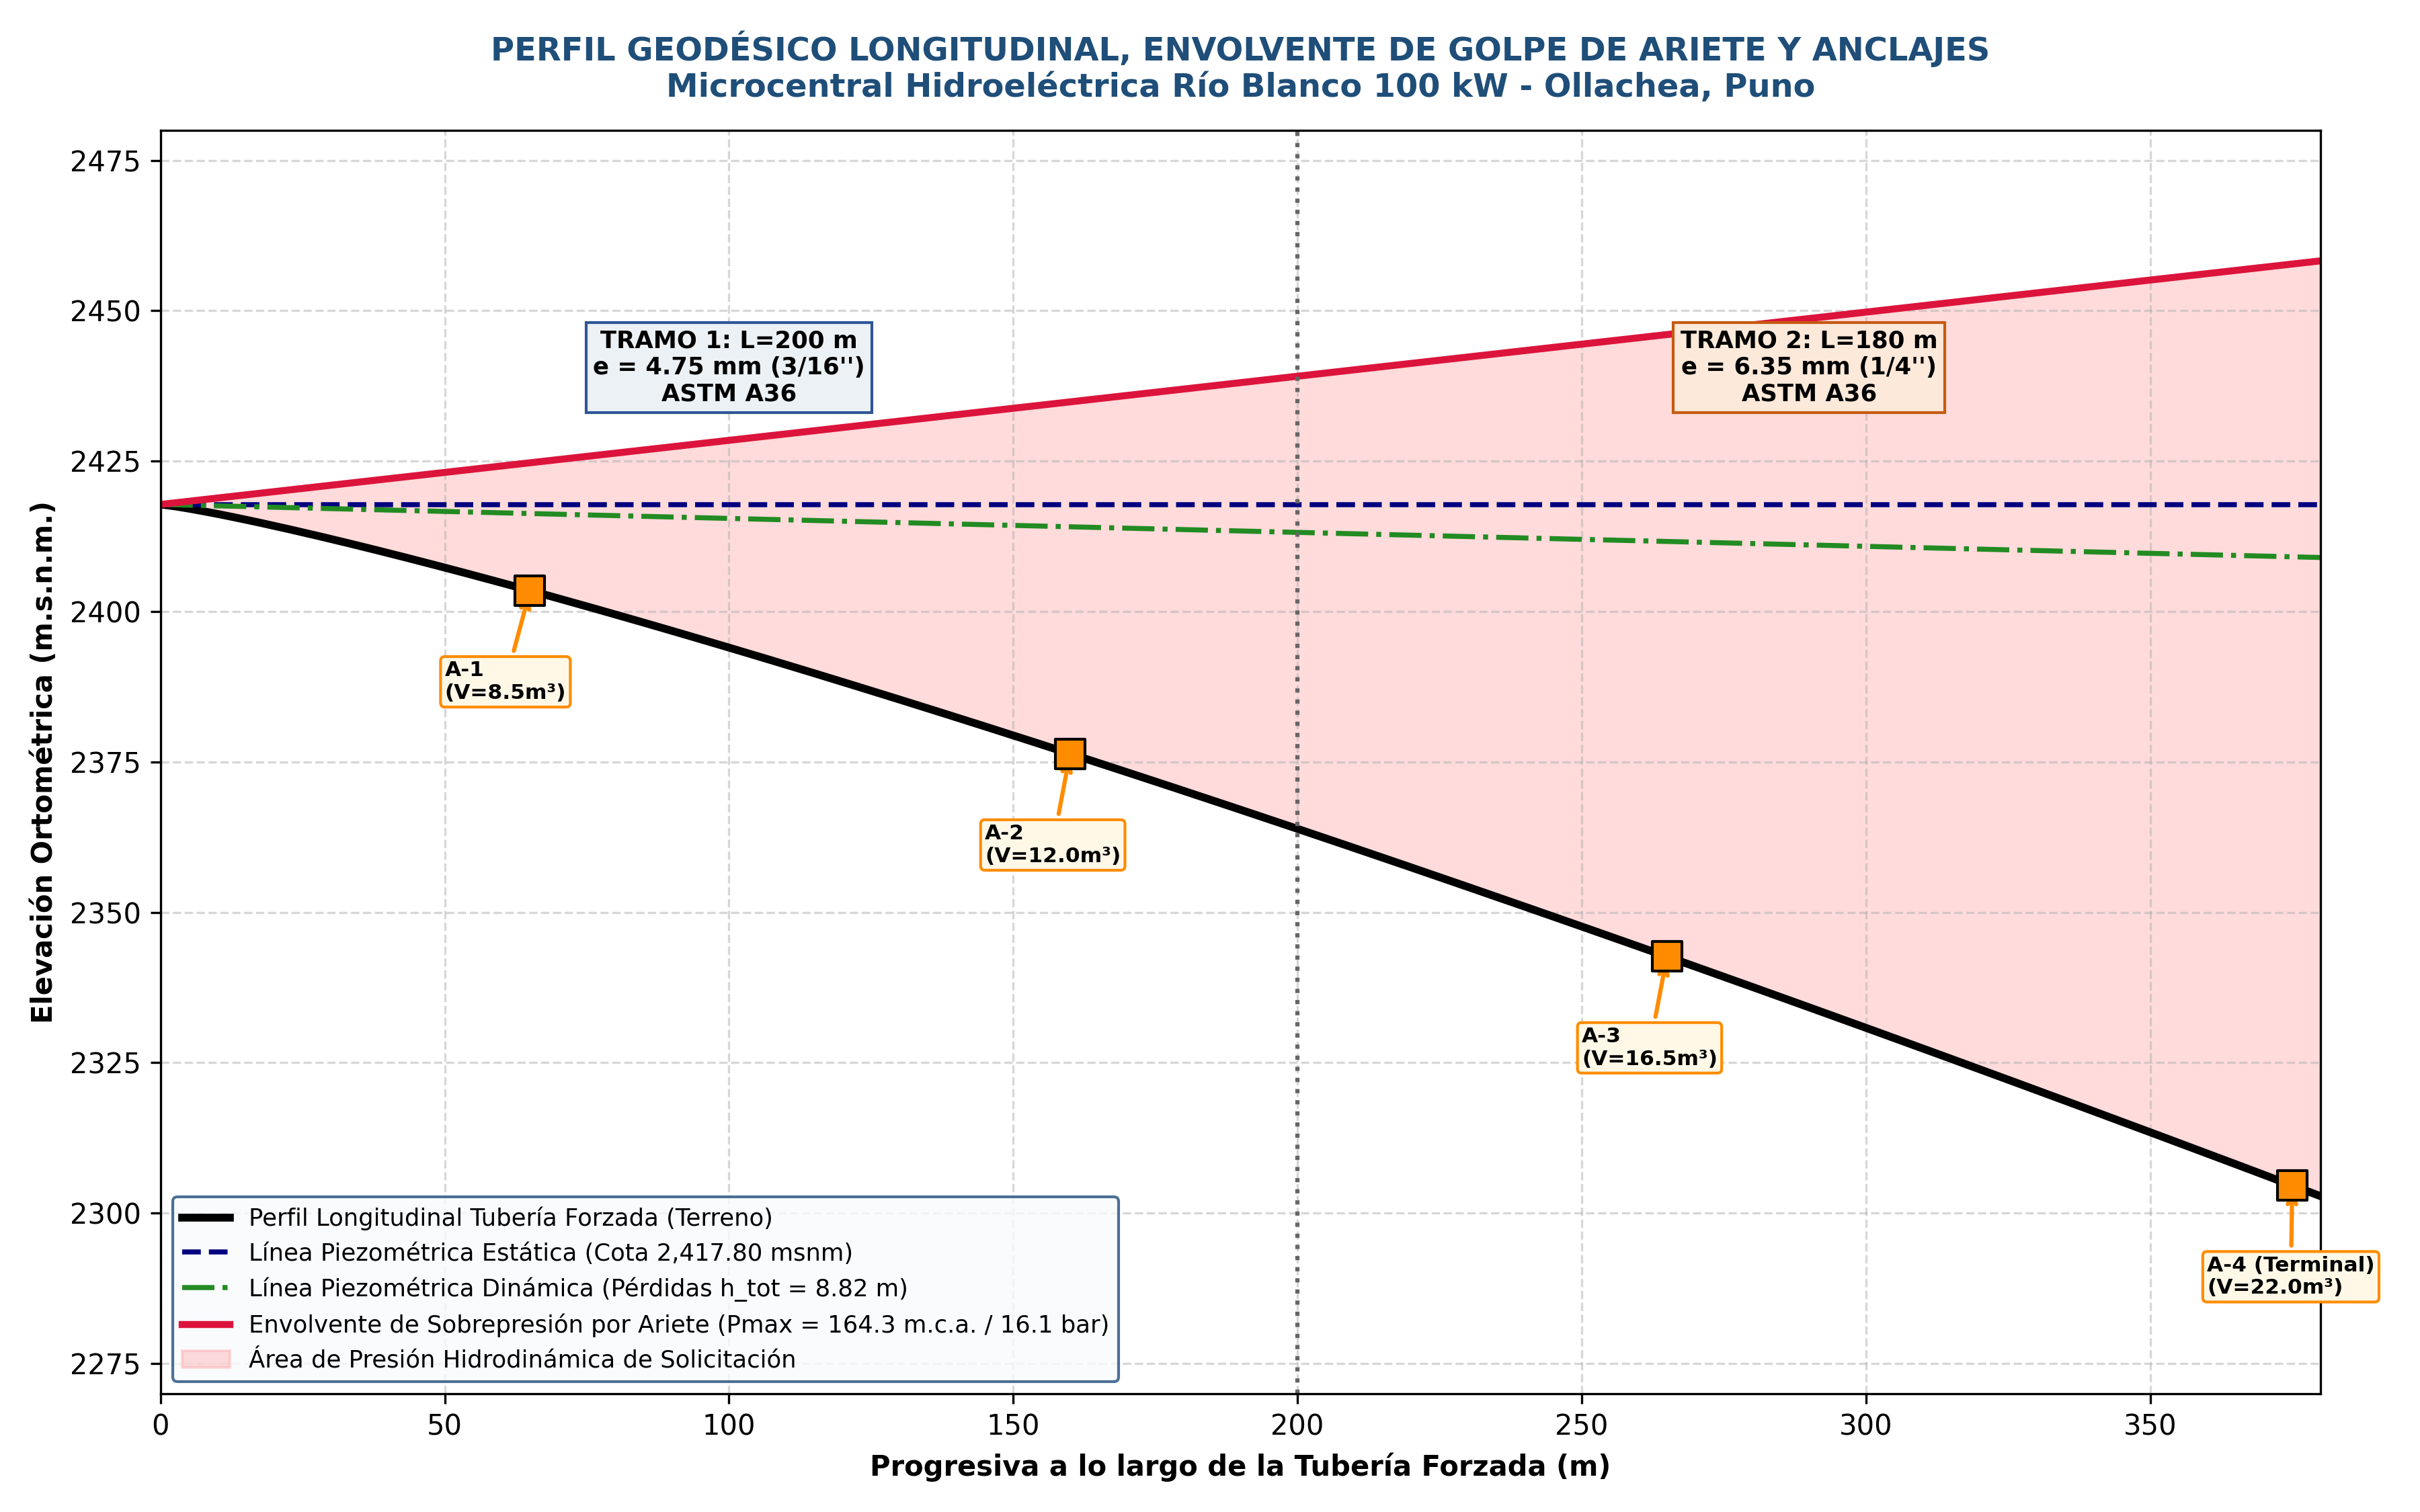
\includegraphics[width=.9\textwidth]{../04 Mapas/Mapa_05_Perfil_Longitudinal_Tuberia_Forzada.png}\caption{Perfil conceptual de tubería forzada; cotas y presión requieren validación.}\end{figure}

\subsection*{7.1 Planos requeridos para la siguiente etapa}
Ubicación y accesos; planta general georreferenciada; captación y desarenador; perfiles y secciones de canal; cámara de carga; tubería, apoyos, válvula y anclajes; casa de máquinas y restitución; unifilar, protecciones, medición, puesta a tierra; subestación y línea en punto aprobado. El Anexo A contiene láminas de gran formato conceptuales.

% CAPÍTULO VIII
\capitulo{VIII}{CONCLUSIONES, RECOMENDACIONES Y BIBLIOGRAFÍA}
\subsection*{8.1 Conclusiones técnicas}
\begin{enumerate}
\item La configuración Pelton para salto alto es una alternativa de estudio, pero la topografía, geología y condiciones reales del cauce no se han acreditado en campo.
\item En la serie provisional, Q95 menos reserva de 30 L/s deja 96 L/s, menos que el caudal nominal de 125 L/s. No se demuestra que el diseño pueda operar a plena carga con la persistencia indicada.
\item El punto de potencia calculado da 104,43 kW después del transformador, frente a 100 kW activos de referencia del generador a cos $\varphi=0,80$.
\item Pérdidas singulares, diámetro económico, eficiencia anual, espesores y anclajes muestran discrepancias o requieren verificación; los resultados no cierran una ingeniería de detalle.
\item La energía, demanda y evaluación financiera son escenarios. No hay datos suficientes para concluir viabilidad, bancabilidad ni beneficios comunitarios comprometidos.
\end{enumerate}

\subsection*{8.2 Recomendaciones}
Contratar primero Gate 0; obtener serie primaria y aforos trazables; consultar a ANA por disponibilidad, caudal ecológico, obras y derechos; levantar topografía/geodesia; inspeccionar geología y geotecnia; confirmar crecidas y sedimentos; revisar demanda y acuerdos locales; pedir condiciones de conexión a la distribuidora; y rehacer cálculos/economía con una única base de diseño antes de factibilidad. Los planos y especificaciones deben ser desarrollados y firmados por profesionales responsables.

\subsection*{8.3 Bibliografía y fuentes de trabajo}
\begin{itemize}
\item Repositorio del proyecto, archivos de datos, scripts, informes y anexos: \url{https://github.com/gaelrenzo/Estudio_microcentral_100_kW_Puno}.
\item Autoridad Nacional del Agua. Resolución Jefatural N.° 267-2019-ANA, lineamientos generales para determinar caudales ecológicos: \url{https://www.gob.pe/institucion/ana/normas-legales/537631-rj-267-2019-ana}.
\item MINEM. R.M. N.° 0214-2011-MEM, Código Nacional de Electricidad (Suministro 2011): \url{https://www.gob.pe/institucion/minem/normas-legales/108753-0214-2011-mem}.
\item D.S. N.° 014-2019-EM, Reglamento para la Protección Ambiental en las Actividades Eléctricas: \url{https://sinia.minam.gob.pe/normas/reglamento-proteccion-ambiental-las-actividades-electricas}.
\item Ley N.° 29338, Ley de Recursos Hídricos y normas complementarias; verificar texto vigente y procedimiento aplicable.
\end{itemize}
Las referencias orientan el análisis; no son pronunciamiento de la autoridad ni sustituyen la verificación normativa al tramitar.

% CAPÍTULO IX
\capitulo{IX}{PRESUPUESTO ESTIMADO}
\subsection*{9.1 Resumen CAPEX del Anexo D}
\begin{table}[H]\centering\small
\begin{tabularx}{\textwidth}{Yrr}\toprule Componente & USD & Participación\\\midrule
Captación, azud, rejilla y desarenador & 42 500 & 17,3\%\\
Canal de aducción, 450 m & 42 000 & 17,1\%\\
Cámara, aliviadero y cuatro anclajes & 26 800 & 10,9\%\\
Tubería de acero, 250 mm × 380 m & 43 500 & 17,7\%\\
Turbina, válvula y ELC & 45 000 & 18,3\%\\
Generador, control y tierra & 16 500 & 6,7\%\\
Subestación y línea MT de referencia & 14 500 & 5,9\%\\
Ingeniería y supervisión & 8 500 & 3,5\%\\
Gestión ambiental, permisos y contingencia preliminar & 6 500 & 2,6\%\\\midrule
\textbf{TOTAL REFERENCIAL} & \textbf{245 800} & \textbf{100\%}\\\bottomrule
\end{tabularx}\caption{Resumen CAPEX académico, no oferta ni cotización.}\end{table}

\subsection*{9.2 Detalle de partidas del APU del Anexo D}
La siguiente transcripción facilita la lectura del presupuesto de trabajo. Las partidas, cantidades y precios unitarios provienen del archivo Excel del Anexo D y requieren revisión de metrado, mercado y alcance.
\begin{longtable}{p{.8cm}p{6.0cm}p{.8cm}r r r}
\caption{Detalle de partidas y costos del APU de referencia (USD).}\\
\toprule Ítem & Descripción & Und. & Metrado & P.U. & Parcial\\\midrule\endfirsthead
\toprule Ítem & Descripción & Und. & Metrado & P.U. & Parcial\\\midrule\endhead
\multicolumn{6}{l}{\textbf{01.00 Obras civiles preliminares y bocatoma}}\\
01.01 & Limpieza, desbroce y trazo geodésico & m$^2$ & 1 500 & 3,50 & 5 250\\
01.02 & Excavación en roca para azud & m$^3$ & 185 & 48,00 & 8 880\\
01.03 & Concreto ciclópeo en azud & m$^3$ & 65 & 135,00 & 8 775\\
01.04 & Rejilla Coanda AISI 304 & und & 1 & 5 500,00 & 5 500\\
01.05 & Compuerta plana de captación y limpia & und & 2 & 2 800,00 & 5 600\\
\multicolumn{6}{l}{\textbf{02.00 Desarenador de doble nave}}\\
02.01 & Excavación de desarenador & m$^3$ & 120 & 28,00 & 3 360\\
02.02 & Concreto armado del desarenador & m$^3$ & 32 & 240,00 & 7 680\\
02.03 & Acero corrugado grado 60 & kg & 2 400 & 2,10 & 5 040\\
02.04 & Vertederos Sutro y compuertas de purga & glb & 1 & 4 500,00 & 4 500\\
\multicolumn{6}{l}{\textbf{03.00 Canal de aducción rectangular}}\\
03.01 & Excavación en roca/material semiduro & m$^3$ & 380 & 35,00 & 13 300\\
03.02 & Concreto ciclópeo para canal 0,50 × 0,60 m & m$^3$ & 115 & 160,00 & 18 400\\
03.03 & Juntas elastoméricas premoldeadas & m & 150 & 18,00 & 2 700\\
03.04 & Muros y banquetas de protección & m & 90 & 84,44 & 7 600\\
\multicolumn{6}{l}{\textbf{04.00 Cámara, aliviadero y anclajes}}\\
04.01 & Excavación de explanada de cámara & m$^3$ & 95 & 26,00 & 2 470\\
04.02 & Concreto armado de cámara de carga & m$^3$ & 28 & 250,00 & 7 000\\
04.03 & Rejilla fina y compuerta de admisión & glb & 1 & 4 800,00 & 4 800\\
04.04 & Concreto de cuatro bloques de anclaje & m$^3$ & 59 & 145,00 & 8 555\\
04.05 & Tubo anti-vacío galvanizado DN 100 & und & 1 & 1 175,00 & 1 175\\
\multicolumn{6}{l}{\textbf{05.00 Tubería forzada (D=250 mm, L=380 m)}}\\
05.01 & Penstock ASTM A36, espesor 4,75 mm, tramo 0--200 m & m & 200 & 95,00 & 19 000\\
05.02 & Penstock ASTM A36, espesor 6,35 mm, tramo 200--380 m & m & 180 & 120,00 & 21 600\\
05.03 & Juntas Dresser de alta presión & und & 4 & 725,00 & 2 900\\
\multicolumn{6}{l}{\textbf{06.00 Equipamiento electromecánico}}\\
06.01 & Turbina Pelton dos inyectores, rodete CA6NM & und & 1 & 28 500,00 & 28 500\\
06.02 & Válvula esférica de guarda DN 200 & und & 1 & 6 500,00 & 6 500\\
06.03 & ELC PWM y banco resistivo de 120 kW & und & 1 & 10 000,00 & 10 000\\
06.04 & Generador síncrono brushless de 125 kVA & und & 1 & 12 500,00 & 12 500\\
06.05 & Tablero, sincronización y protecciones & und & 1 & 4 000,00 & 4 000\\
\multicolumn{6}{l}{\textbf{07.00 Subestación y línea de media tensión}}\\
07.01 & Transformador 125 kVA, 0,38/10 kV ONAN & und & 1 & 8 200,00 & 8 200\\
07.02 & Línea aérea 10 kV, AAAC 35 mm$^2$ & km & 3,2 & 1 500,00 & 4 800\\
07.03 & Malla de tierra con ocho jabalinas & glb & 1 & 1 500,00 & 1 500\\
\bottomrule
\end{longtable}
El archivo fuente desglosa costos directos y gastos generales/utilidad en hojas adicionales; el resumen de inversión de USD 245 800 no se ha cotizado ni contrastado en mercado.

\subsection*{9.3 Costos de operación y evaluación de escenario}
El OPEX anual se toma como 3\% del CAPEX, es decir USD 7 374. Con energía de 862,92 MWh/año y tarifa de USD 0,075/kWh, los ingresos brutos modelados son cerca de USD 64 720/año. El flujo operativo simplificado es USD 57 346/año. A 25 años y 10\% de descuento, la evaluación reporta VAN USD 274 742, TIR 23,20\%, recuperación simple 4,29 años, LCOE USD 39,90/MWh y B/C 1,88.

\begin{alertabox}[title=Alcance económico]
No se presentan cotizaciones trazables ni un diseño con metrados validados. Deben incluirse impuestos, transporte, campamento, conexión, permisos, servidumbres, contingencias, reposición de equipos, seguros, personal, depreciación, financiamiento y tarifa/contrato. Los indicadores no son recomendación de inversión.
\end{alertabox}

\subsection*{9.4 Sensibilidad de escenario disponible}
La matriz publicada incluye: CAPEX +20\% (VAN USD 212 195, TIR 18,68\%); CAPEX --20\% (USD 337 288, 29,87\%); tarifa +20\% (USD 392 237, 28,54\%); tarifa --20\% (USD 157 247, 17,76\%); energía --25\% (USD 127 873, 16,37\%); escenario adverso combinado (VAN --USD 22 795, TIR 8,98\%, B/C 0,94); escenario favorable combinado (USD 461 696, 33,99\%, B/C 2,64). Son variaciones deterministas de entradas supuestas, no probabilidades ni resultados P50/P90. El archivo CSV de sensibilidad está en \path{data/sensibilidad_extrema.csv}.

% CAPÍTULO X
\capitulo{X}{ESPECIFICACIONES TÉCNICAS DE PARTIDAS}
Estas descripciones estructuran partidas para el siguiente expediente. Las unidades, cantidades, controles, métodos y tolerancias deben ajustarse con planos aprobados, norma aplicable y condiciones del sitio.

\subsection*{10.1 Obras preliminares y movimiento de tierras}
Incluye movilización, señalización, instalaciones temporales, control topográfico, acceso autorizado, desbroce limitado, excavación, clasificación de material, perfilado, drenaje, carga, transporte y disposición en lugar autorizado. Medición por área/volumen aprobado, con secciones previas y posteriores. No iniciar sin límites de predio, servidumbres y seguridad definidos.

\subsection*{10.2 Concreto y obras hidráulicas}
Incluye preparación de fundaciones, encofrado, acero, concreto ciclópeo/armado, juntas, curado, azud, desarenador, canal, cámara, aliviadero, rejillas y compuertas. Controlar materiales, asentamiento, probetas, temperatura/curado, cotas, espesor, juntas, estanqueidad y maniobra. Medición por volumen/masa/unidad aceptada. No asumir la resistencia de las fuentes sin diseño estructural.

\subsection*{10.3 Tubería, soldadura y anclajes}
Incluye suministro por diámetro y clase de presión, biseles, soldadura con procedimiento y soldadores aprobados, END, accesorios, válvula, apoyos, silletas, bloques, recubrimiento y prueba hidráulica. Medición por longitud instalada y accesorios aprobados. La presión, vacío, espesor, tolerancias, intervalos de inspección y prueba se fijarán con código y cálculo de transitorios completos.

\subsection*{10.4 Grupo turbina-generador y control}
Incluye transporte, montaje, alineamiento, acoplamiento, válvula, inyectores, gobernador/ELC, excitación, sensores, protecciones, banco resistivo, pruebas de fábrica y puesta en marcha. Aceptación por curvas garantizadas, régimen de embalamiento, vibración, temperatura, regulación de frecuencia/tensión y pruebas de rechazo de carga. Coordinar potencia activa y aparente.

\subsection*{10.5 Instalaciones eléctricas y evacuación}
Incluye transformador, tableros, interruptores, relés, medición, cableado, línea, soportes, protección y puesta a tierra. Antes de instalar, acordar punto de conexión y criterios con operador. Realizar continuidad, aislamiento, relación de transformación, secuencia de fases, pruebas de relé, malla con resistividad medida y prueba de aceptación. Medición por unidad/longitud aprobada.

\subsection*{10.6 Pruebas, recepción y cierre}
Incluye protocolos de pruebas hidráulicas y eléctricas, carga escalonada, disparo, alarmas, parada de emergencia, documentación conforme a obra, manuales, capacitación, manejo de residuos y restauración. La recepción requiere cierre de no conformidades y actas del titular y operador.

% CAPÍTULO XI
\capitulo{XI}{TÉRMINOS DE REFERENCIA}
\subsection*{11.1 Objeto}
Contratar estudios iniciales Gate 0 para reducir la incertidumbre del sitio y decidir si procede financiar la factibilidad. Las coordenadas y trazos entregados por el titular se identifican como conceptos, no como levantamiento, límite predial ni permiso de ingreso. Las ofertas separarán impuestos, viáticos, movilización, plazo, supuestos, exclusiones, vigencia, forma de pago y precios por ampliación.

\subsection*{11.2 Lotes de estudio}
\begin{table}[H]\centering\small
\begin{tabularx}{\textwidth}{p{1.8cm}Y Y}\toprule Lote & Alcance base Gate 0 & Ampliación opcional\\\midrule
A. Topografía & Revisión cartográfica, reconocimiento y levantamiento de decisión en hasta 8 ha; captación, canal conceptual, cámara, tubería, casa de máquinas, restitución y accesos. & Mayor área/ejes, ortofoto, vértices certificados si la autoridad lo requiere.\\
B. Hidrología & Auditoría de fuentes/series; reconocimiento; instalación/lectura inicial si se aprueba; 2--4 aforos iniciales. & Campaña de 12 meses, 15--20 aforos y estudio completo para procedimiento de disponibilidad hídrica.\\
C. Geotecnia & Revisión geológica, reconocimiento, propuesta de emplazamientos/accesos y brechas. & Calicatas/perforaciones, ensayos y recomendaciones de factibilidad, con aprobación previa.\\
\bottomrule\end{tabularx}\caption{Resumen de lotes del TDR Gate 0.}\end{table}

\subsection*{11.3 Entregables y criterios de aceptación}
El postor presentará plan de trabajo, metodología, polígono, CRS, cronograma, riesgos de campo y permisos; datos crudos editables, metadatos, precisión/incertidumbre, bitácoras y control de calidad; perfiles, secciones y planos; ficha de cada aforo con fecha, equipo, método y condición; diagnóstico geológico-geotécnico; informe de brechas; y recomendación de continuar/no continuar con alcance y costo de fase siguiente. Las ofertas se compararán por trazabilidad, experiencia, seguridad, calidad, alcance desglosado y plazo.

\subsection*{11.4 Seguridad y restricciones}
No se permite ingresar a predios, excavar, tomar muestras, instalar sensores permanentes ni intervenir el cauce sin autorización. El contratista debe coordinar con titular/comunidad, contar con EPP y plan de emergencias, y detener el trabajo ante crecida, clima o acceso inseguro. Los permisos ambientales, hídricos, arqueológicos o prediales se identificarán y no se asumirán obtenidos.

\subsection*{11.5 Documento contractual de referencia}
El texto completo de los términos de referencia, sus cantidades opcionales y criterios de evaluación se incorpora como anexo reproducido. El resumen de este capítulo no lo modifica ni constituye adjudicación.

% ANEXOS ORIGINALES
\clearpage\section*{ANEXOS DE RESPALDO DISPONIBLES}\addcontentsline{toc}{section}{Anexos de respaldo disponibles}
\begin{resumenbox}[title=Nota de lectura de anexos]
Los anexos siguientes se incorporan desde los archivos de trabajo disponibles. La inclusión permite revisar su contenido y trazabilidad documental; no valida los datos que el anexo declara ni sustituye verificación independiente. El Anexo D permanece como hoja de cálculo Excel y sus partidas principales se transcriben en capítulos VI y IX.
\end{resumenbox}

\apendice{A}{Cartografía y planos de gran formato}
Material conceptual. No replantear ni construir sin levantamiento, revisión y firma.
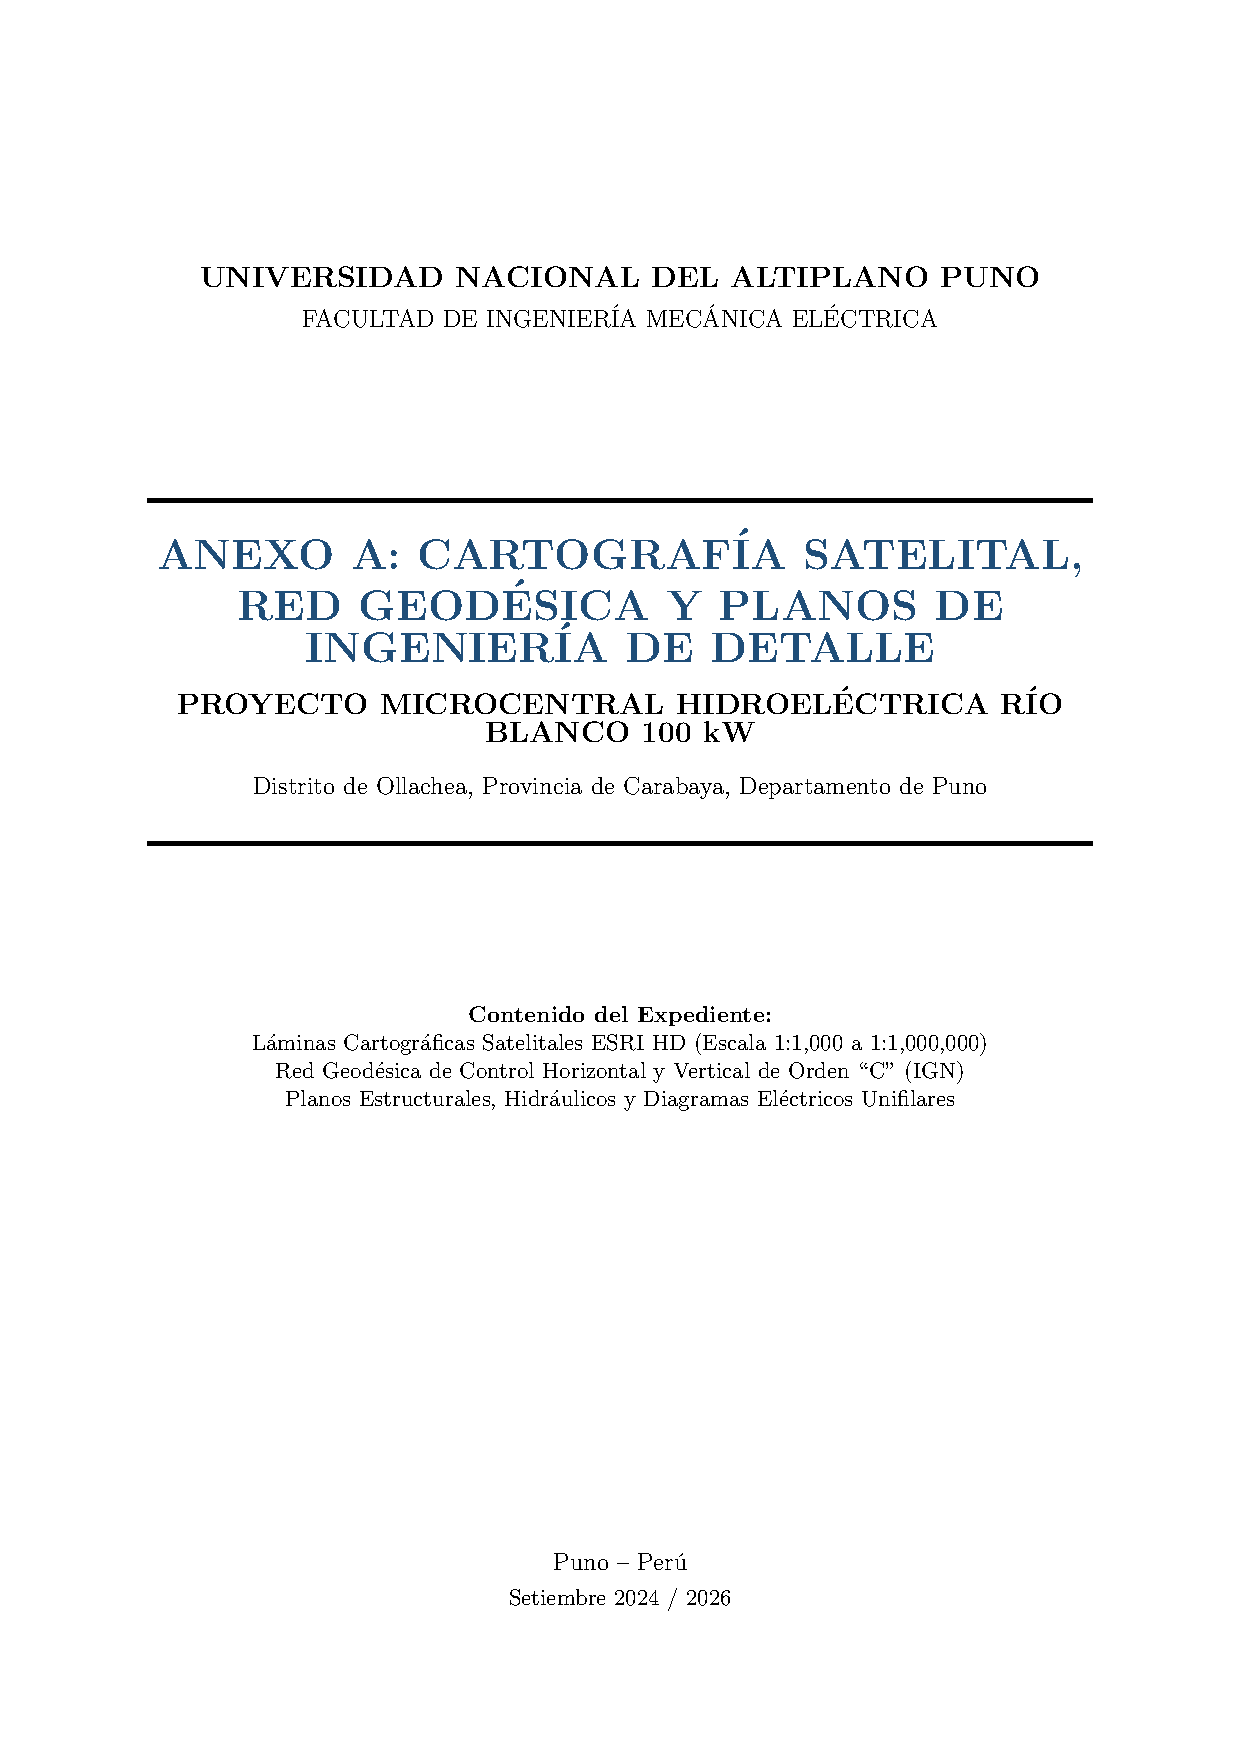
\includepdf[pages=-,fitpaper=true,pagecommand={\thispagestyle{empty}}]{../06 Anexos/Anexo_A_Cartografia_y_Planos_Gran_Formato.pdf}

\apendice{B}{Registro hidrometeorológico extenso}
Resumen de trabajo. La procedencia primaria debe acreditarse antes de usar datos para diseño o disponibilidad.
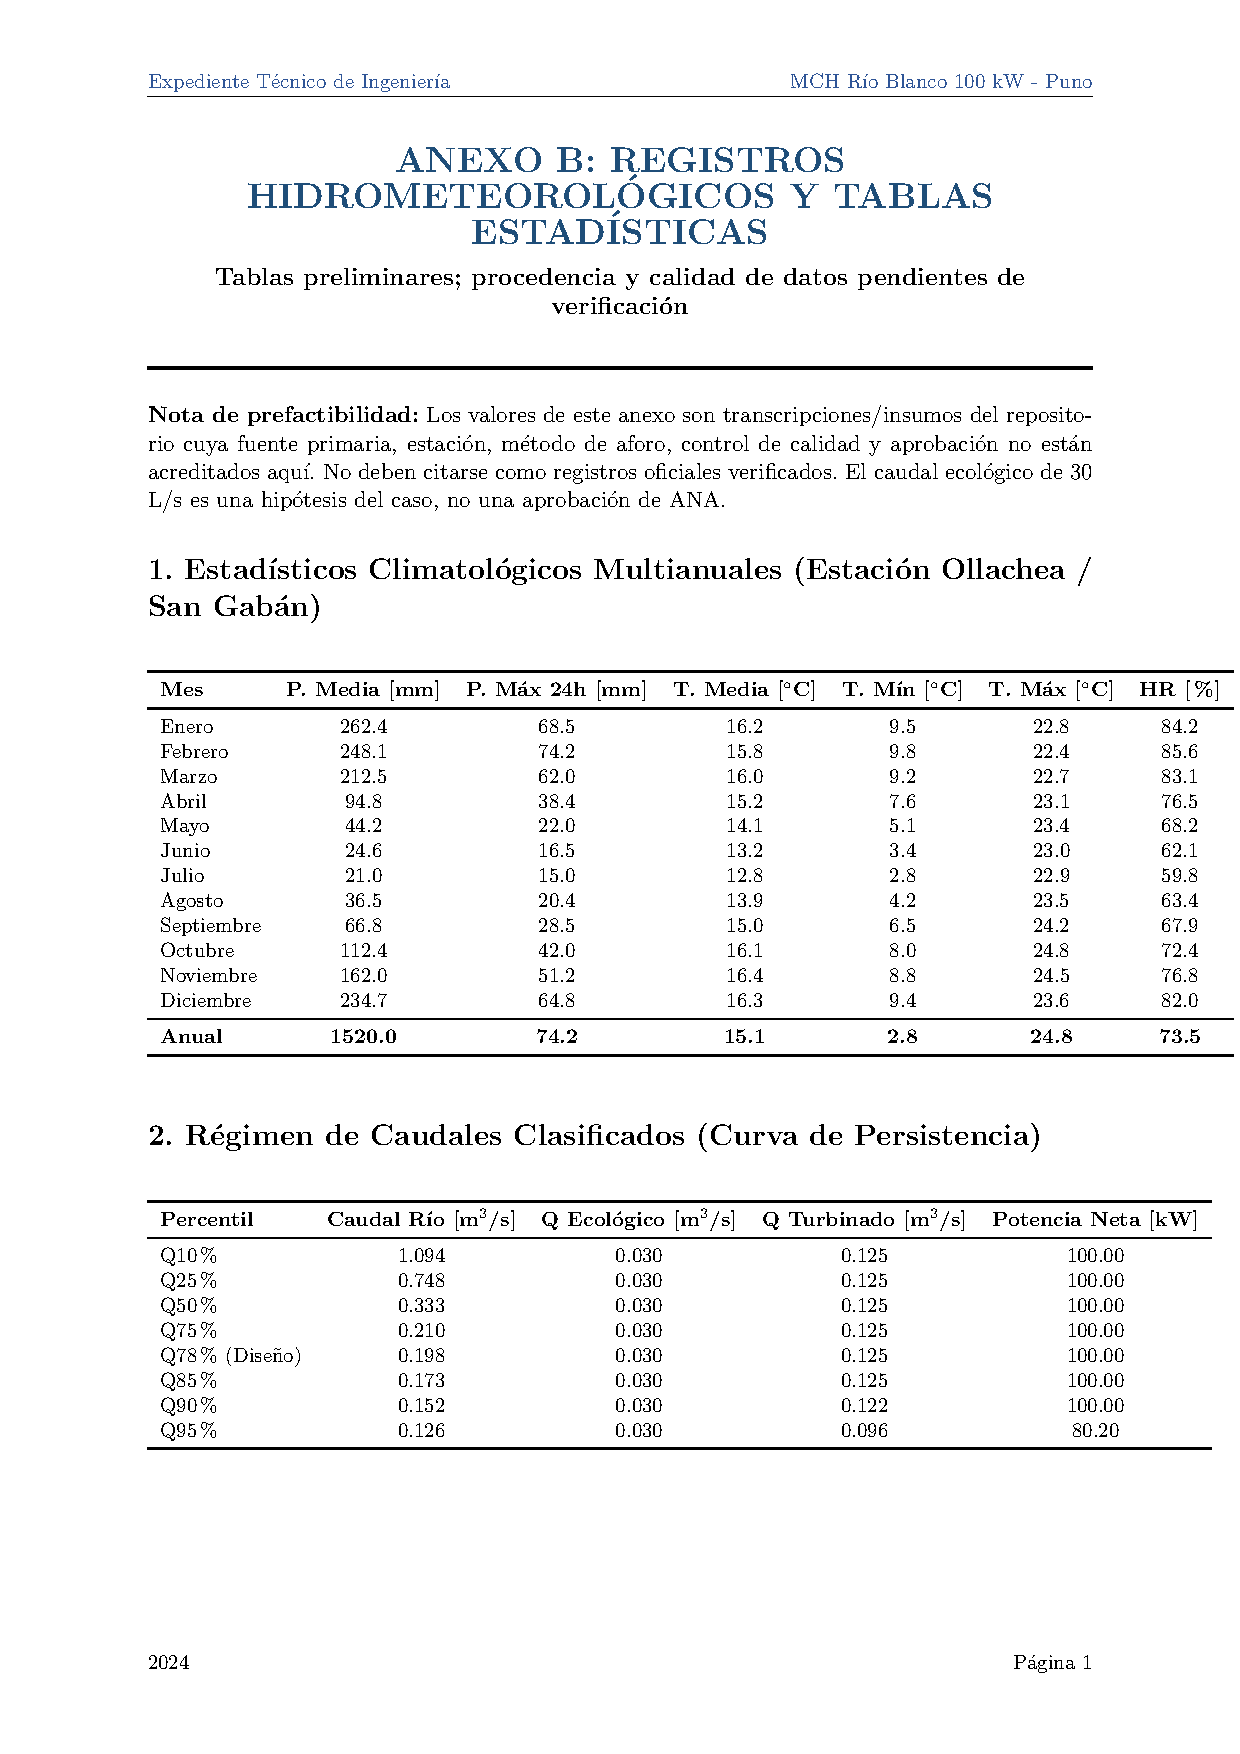
\includepdf[pages=-,fitpaper=true,pagecommand={\thispagestyle{empty}}]{../06 Anexos/Anexo_B_Registro_Hidrometeorologico_Extenso.pdf}

\apendice{C}{Memorias de cálculo hidráulicas y electromecánicas}
Reproducción del anexo fuente. Se identifican discrepancias de pérdidas localizadas, eficiencia y potencia en el capítulo II.
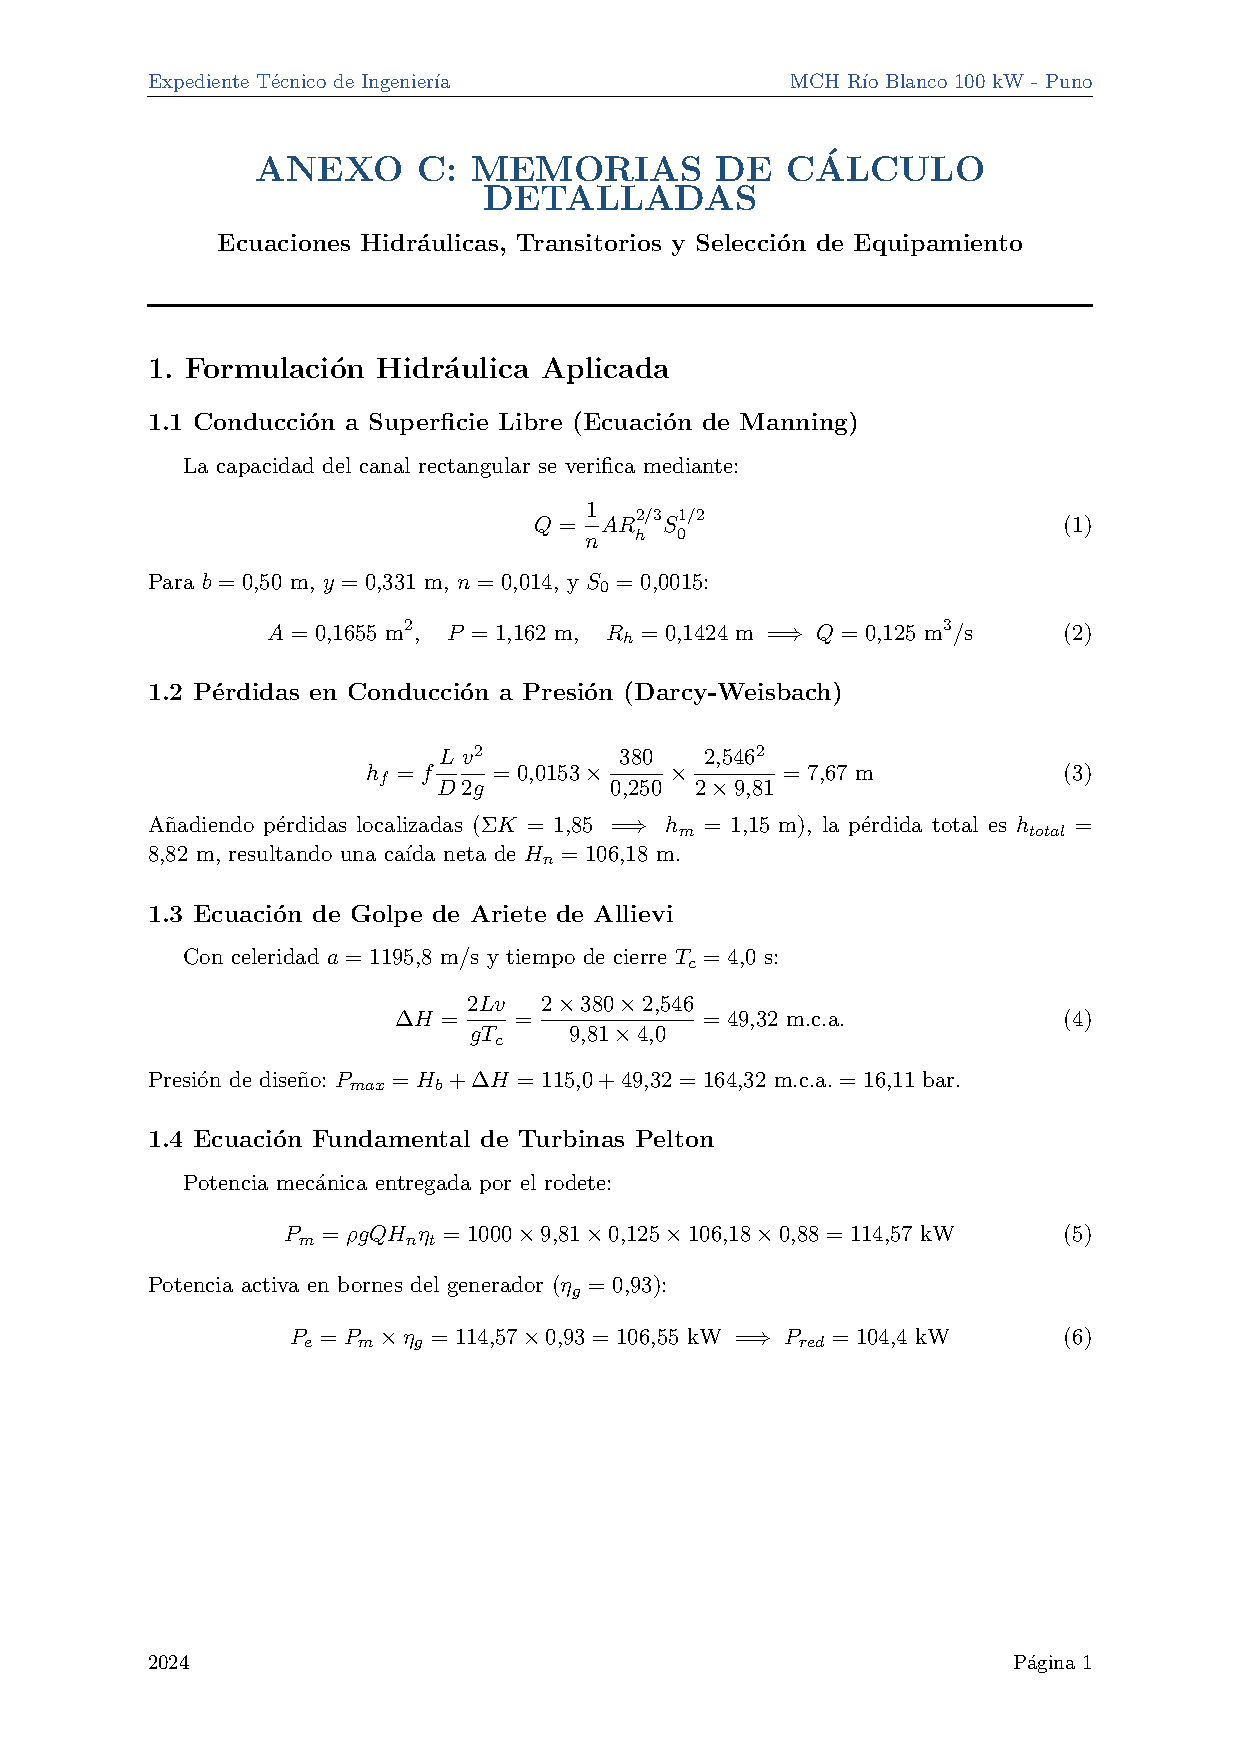
\includepdf[pages=-,fitpaper=true,pagecommand={\thispagestyle{empty}}]{../06 Anexos/Anexo_C_Memorias_Calculo_Detalladas_Hidraulica_y_Electromecanica.pdf}

\apendice{D}{Presupuesto y análisis de precios unitarios}
El archivo fuente es \path{../06 Anexos/Anexo_D_Presupuesto_Analisis_Precios_Unitarios_APU.xlsx}; conservarlo junto con este expediente. Sus precios y metrados son estimativos.

\apendice{E}{Especificaciones de referencia de turbina y generador}
Ficha de referencia no adjudicada; verificar con fabricantes y compatibilidad de potencia.
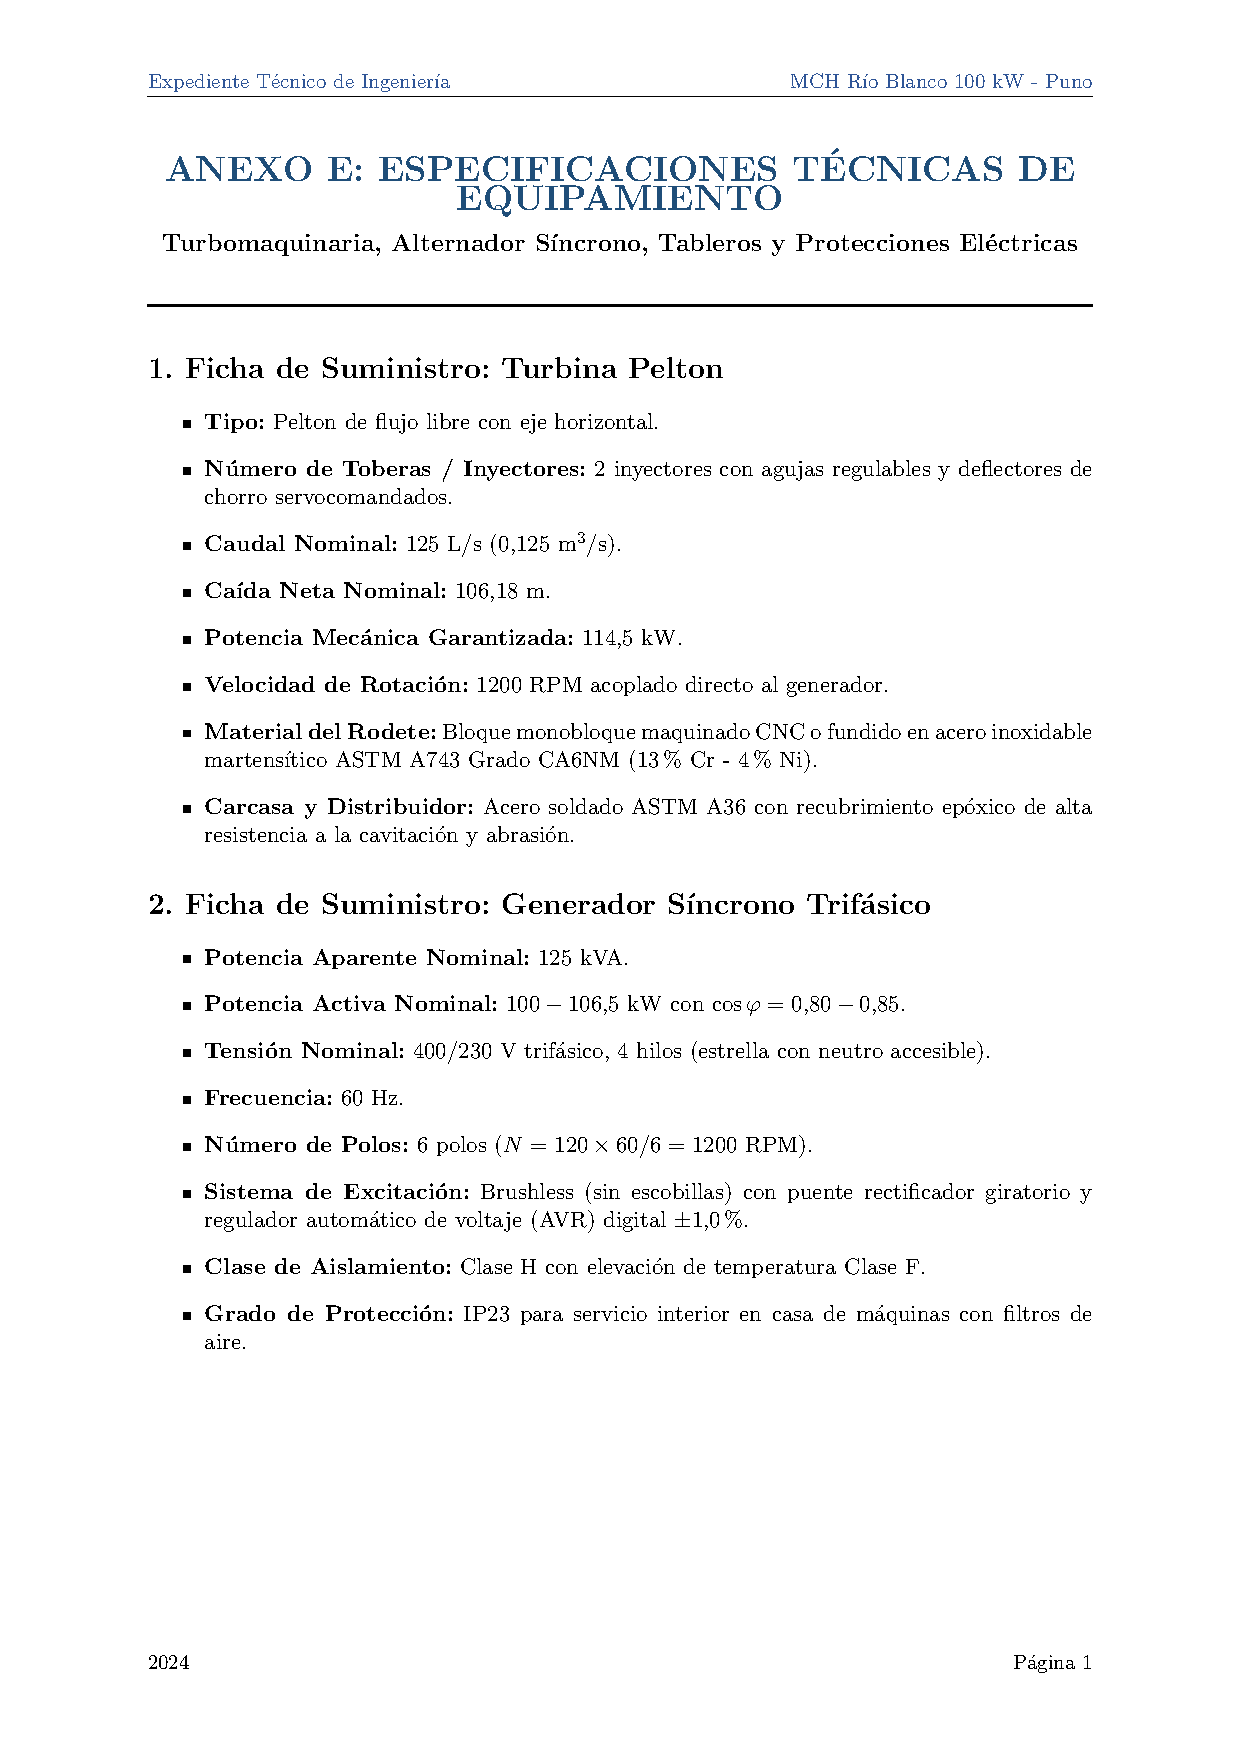
\includepdf[pages=-,fitpaper=true,pagecommand={\thispagestyle{empty}}]{../06 Anexos/Anexo_E_Especificaciones_Tecnicas_Turbina_Pelton_Generador.pdf}

\apendice{F}{Propuesta geodésica y topográfica}
El documento declara que no acredita levantamiento GNSS ni certificación; sus coordenadas de gabinete no son para replanteo.
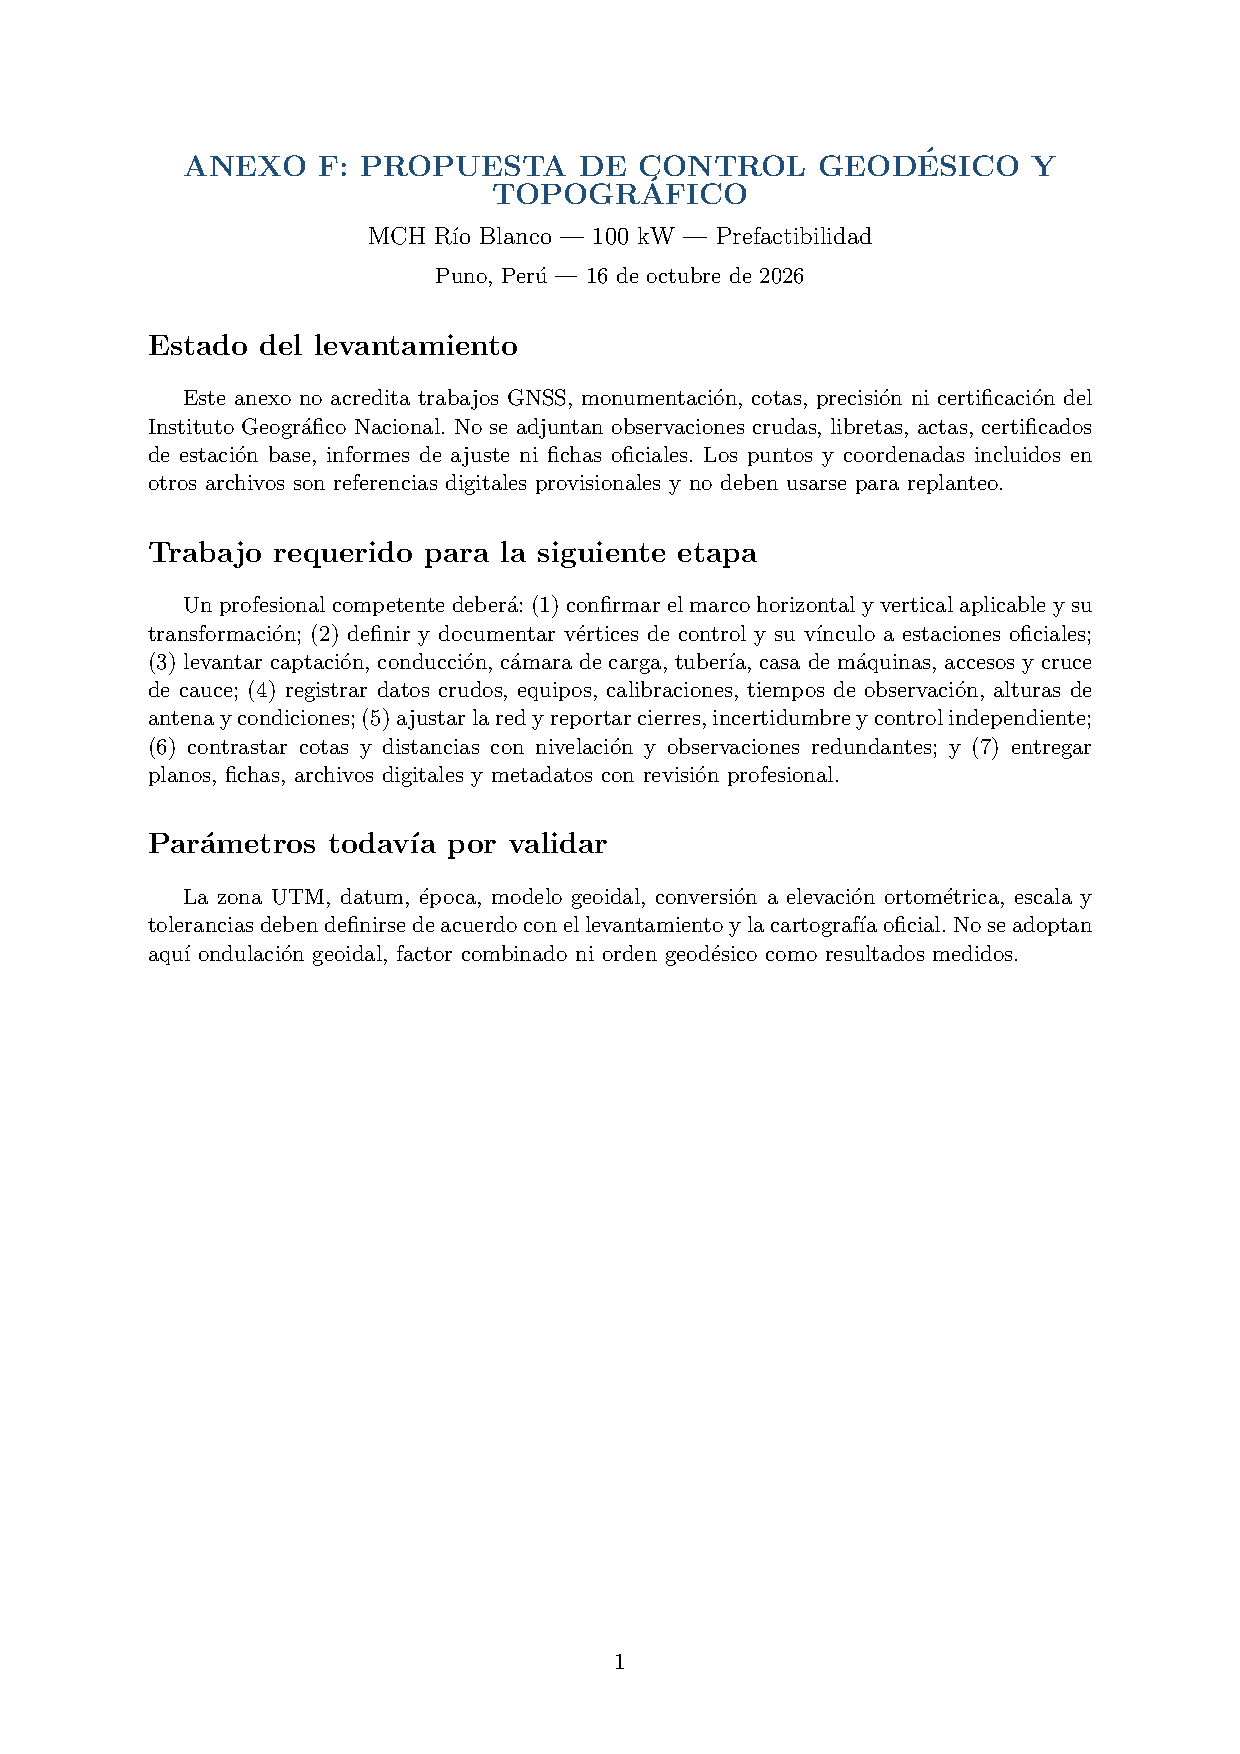
\includepdf[pages=-,fitpaper=true,pagecommand={\thispagestyle{empty}}]{../06 Anexos/Anexo_F_Memoria_Geodesica_y_Topografica.pdf}

\apendice{G}{Usos productivos y desarrollo local}
Hipótesis de aplicaciones y cargas por contrastar mediante consulta a usuarios, encuestas, equipos y acuerdos locales.
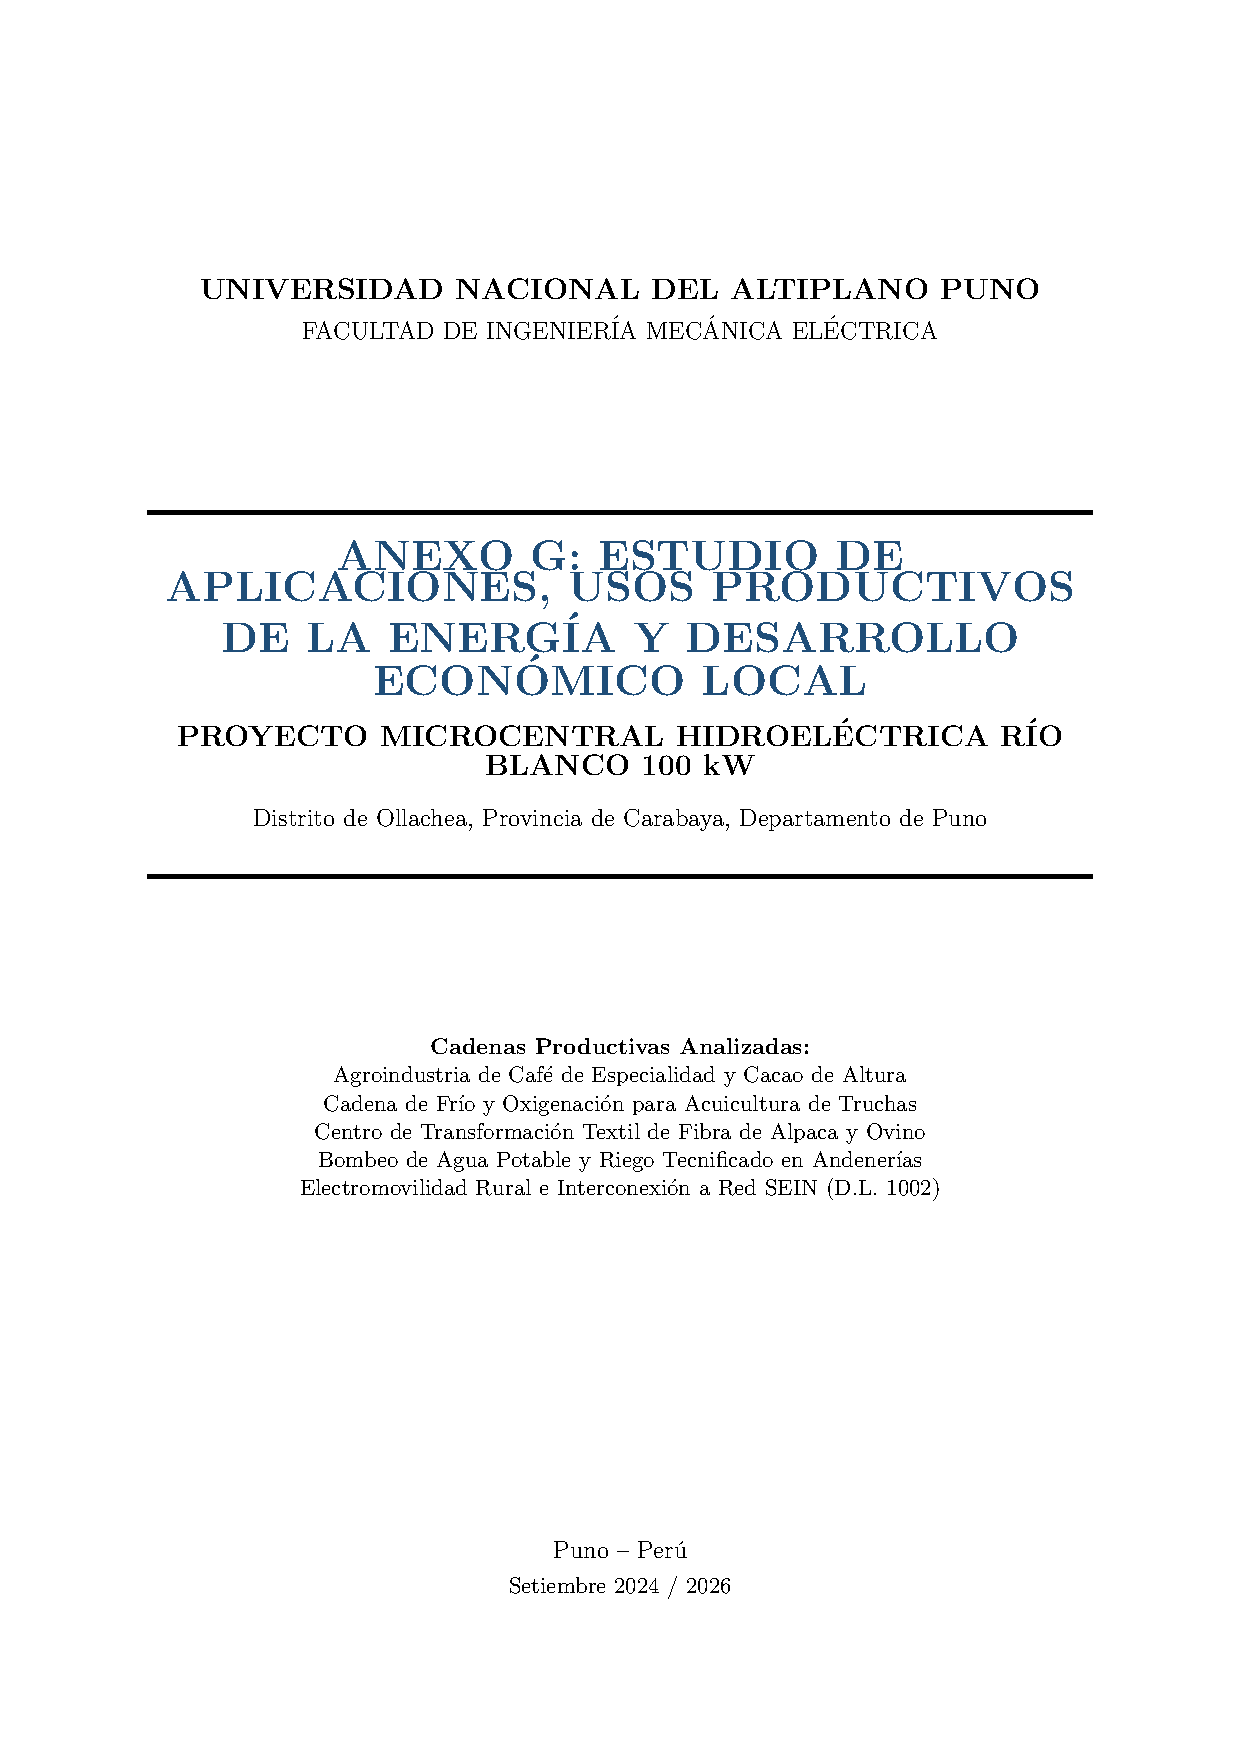
\includepdf[pages=-,fitpaper=true,pagecommand={\thispagestyle{empty}}]{../06 Anexos/Anexo_G_Estudio_Usos_Productivos_y_Desarrollo_Local.pdf}

\apendice{H}{Términos de referencia Gate 0}
Documento completo para solicitar cotizaciones; no es adjudicación ni autorización de trabajos.
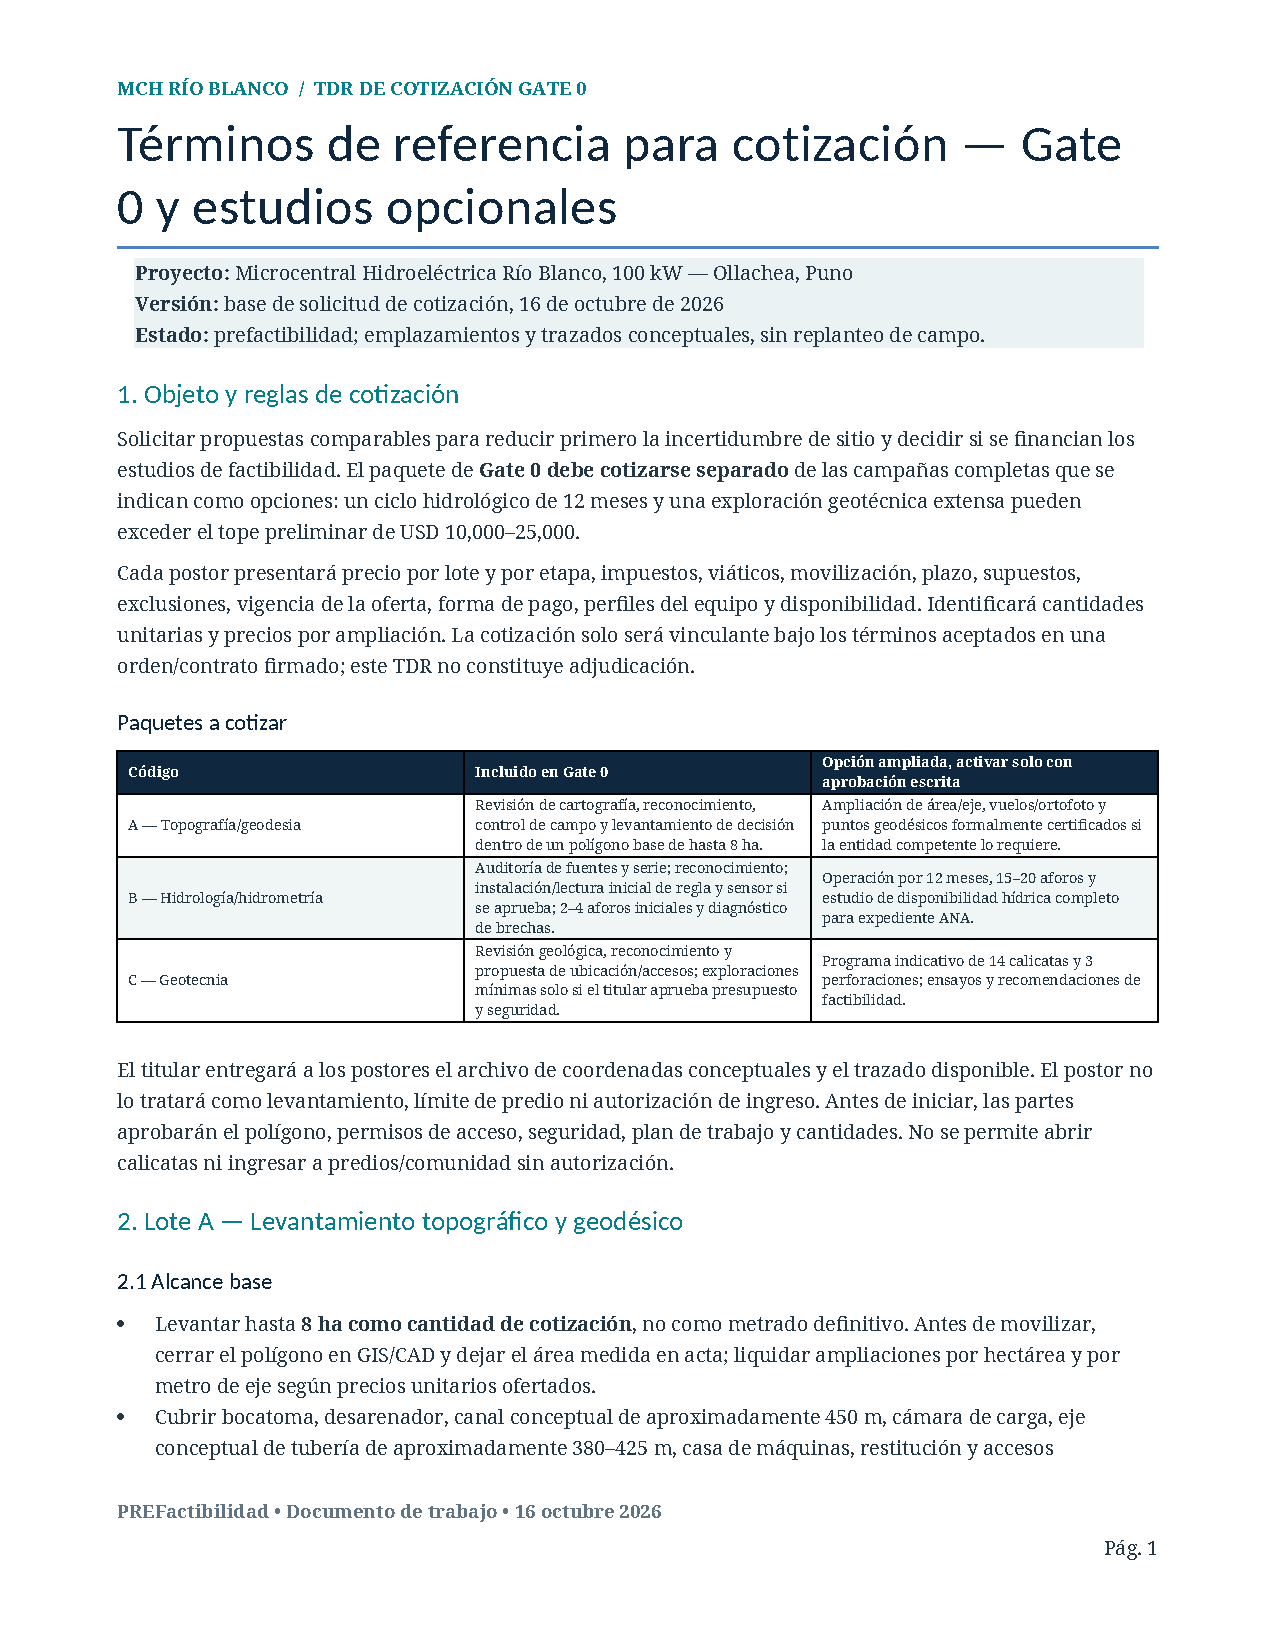
\includepdf[pages=-,fitpaper=true,pagecommand={\thispagestyle{empty}}]{TDR_Estudios_Gate_0.pdf}

\apendice{I}{Decisión Gate 0}
Documento de decisión preliminar y brechas para la siguiente etapa.
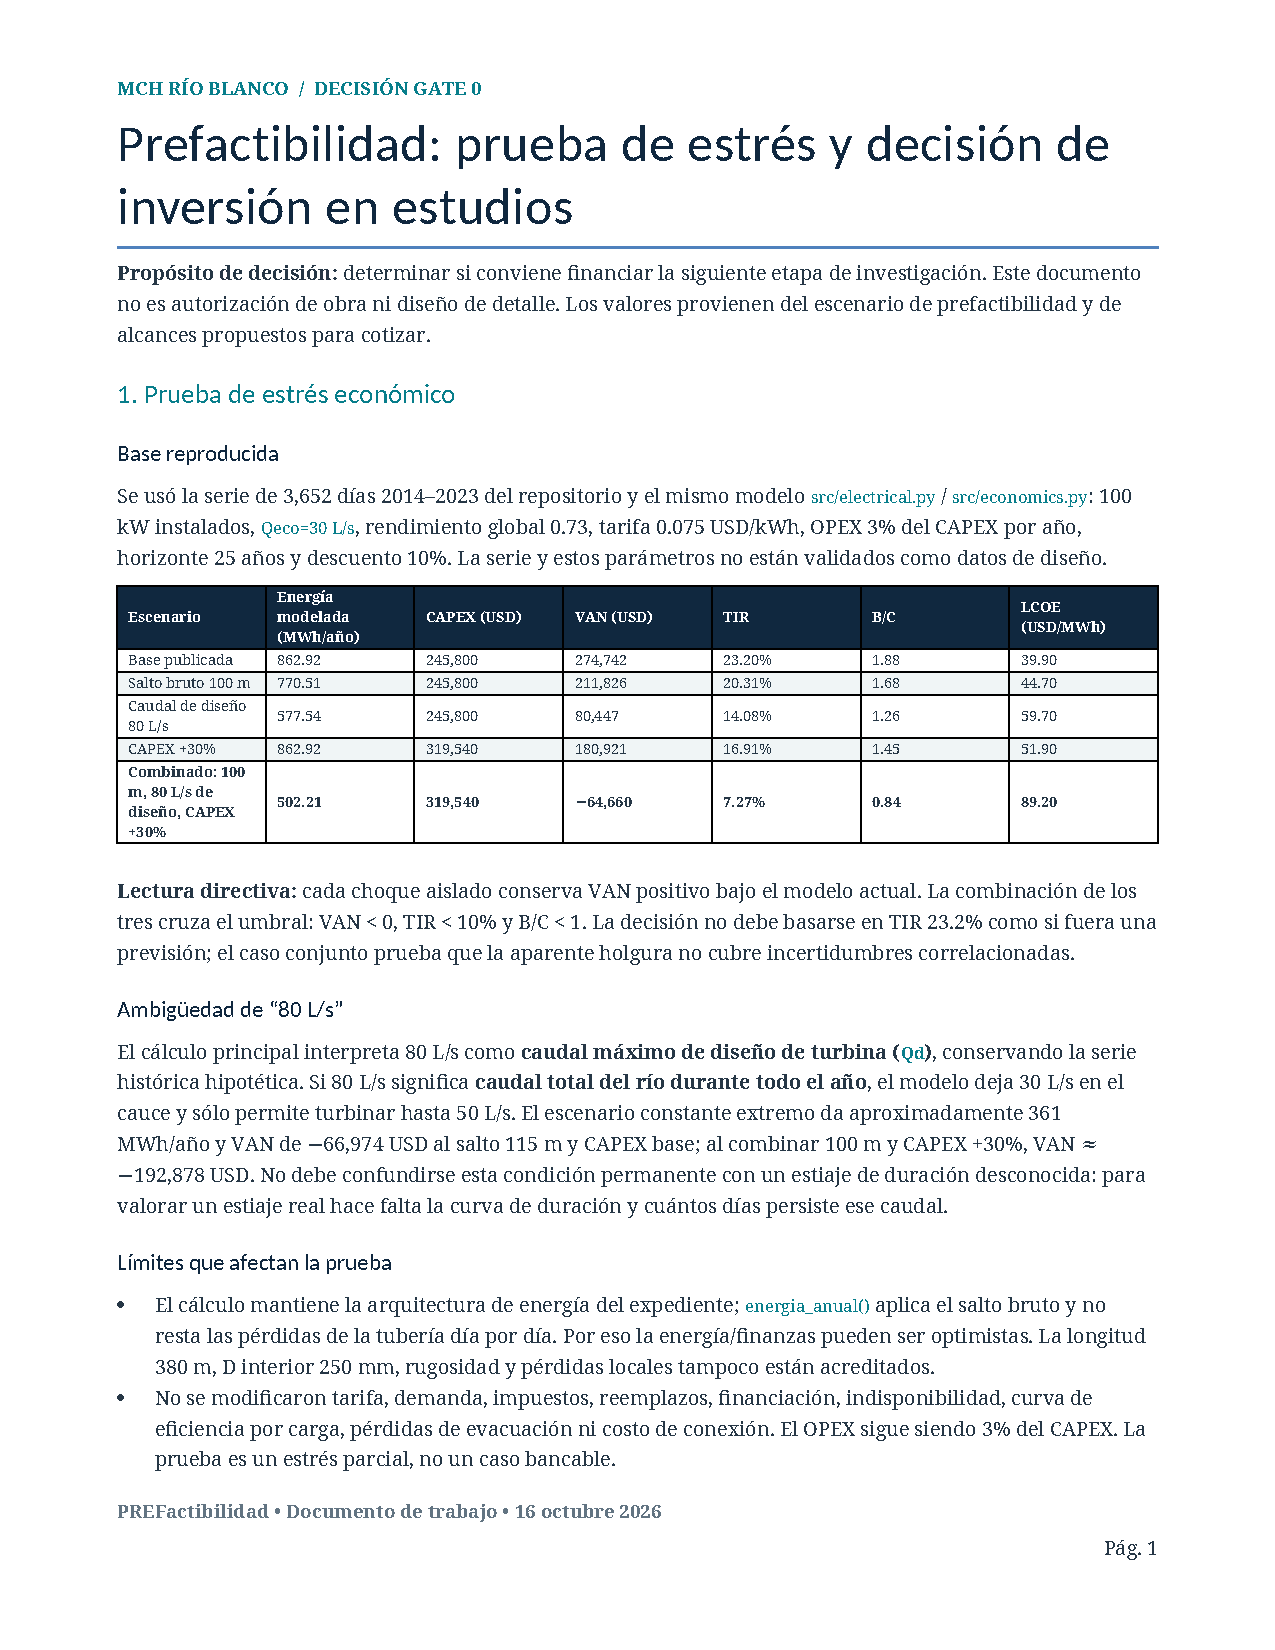
\includepdf[pages=-,fitpaper=true,pagecommand={\thispagestyle{empty}}]{Decision_Gate_0.pdf}

\end{document}
